\section{Исследовательский раздел}
\subsection{Условия исследований}
Исследование проводилось на персональном компьютере со следующими характеристиками:

\begin{itemize}
\item процессор Apple M1 Pro,
\item операционная система macOS Ventura 13.5.2 (22G91),
\item 32 Гб оперативной памяти.
\end{itemize}

Для определения гиперпараметров каждой модели применялся метод поиска по сетке с опорой на значение F1-меры. Разбиение данных на выборки производилось на 4 части, 1 из которых используется в качестве тестовой, результаты приводятся для каждого разбиения.

\subsection{Градиентный бустинг }

Параметры модели при применении метода векторизации ``мешок слов'':
\begin{itemize}
	\item коэффициент обучения -- влияет на скорость обучения -- 0.5;
	\item количество классификаторов в ансамбле -- определяет количество деревьев, используемых в алгоритме -- 215;
	\item минимальное количество образцов для разбиения узла дерева решений -- 5.
\end{itemize}

На рисунке \ref{img:gradientMatrBag} представлены матрицы ошибок, полученные с использованием градиентного бустинга, метод векторизации -- ``мешок слов''.
\begin{figure}[H]
	\centering
	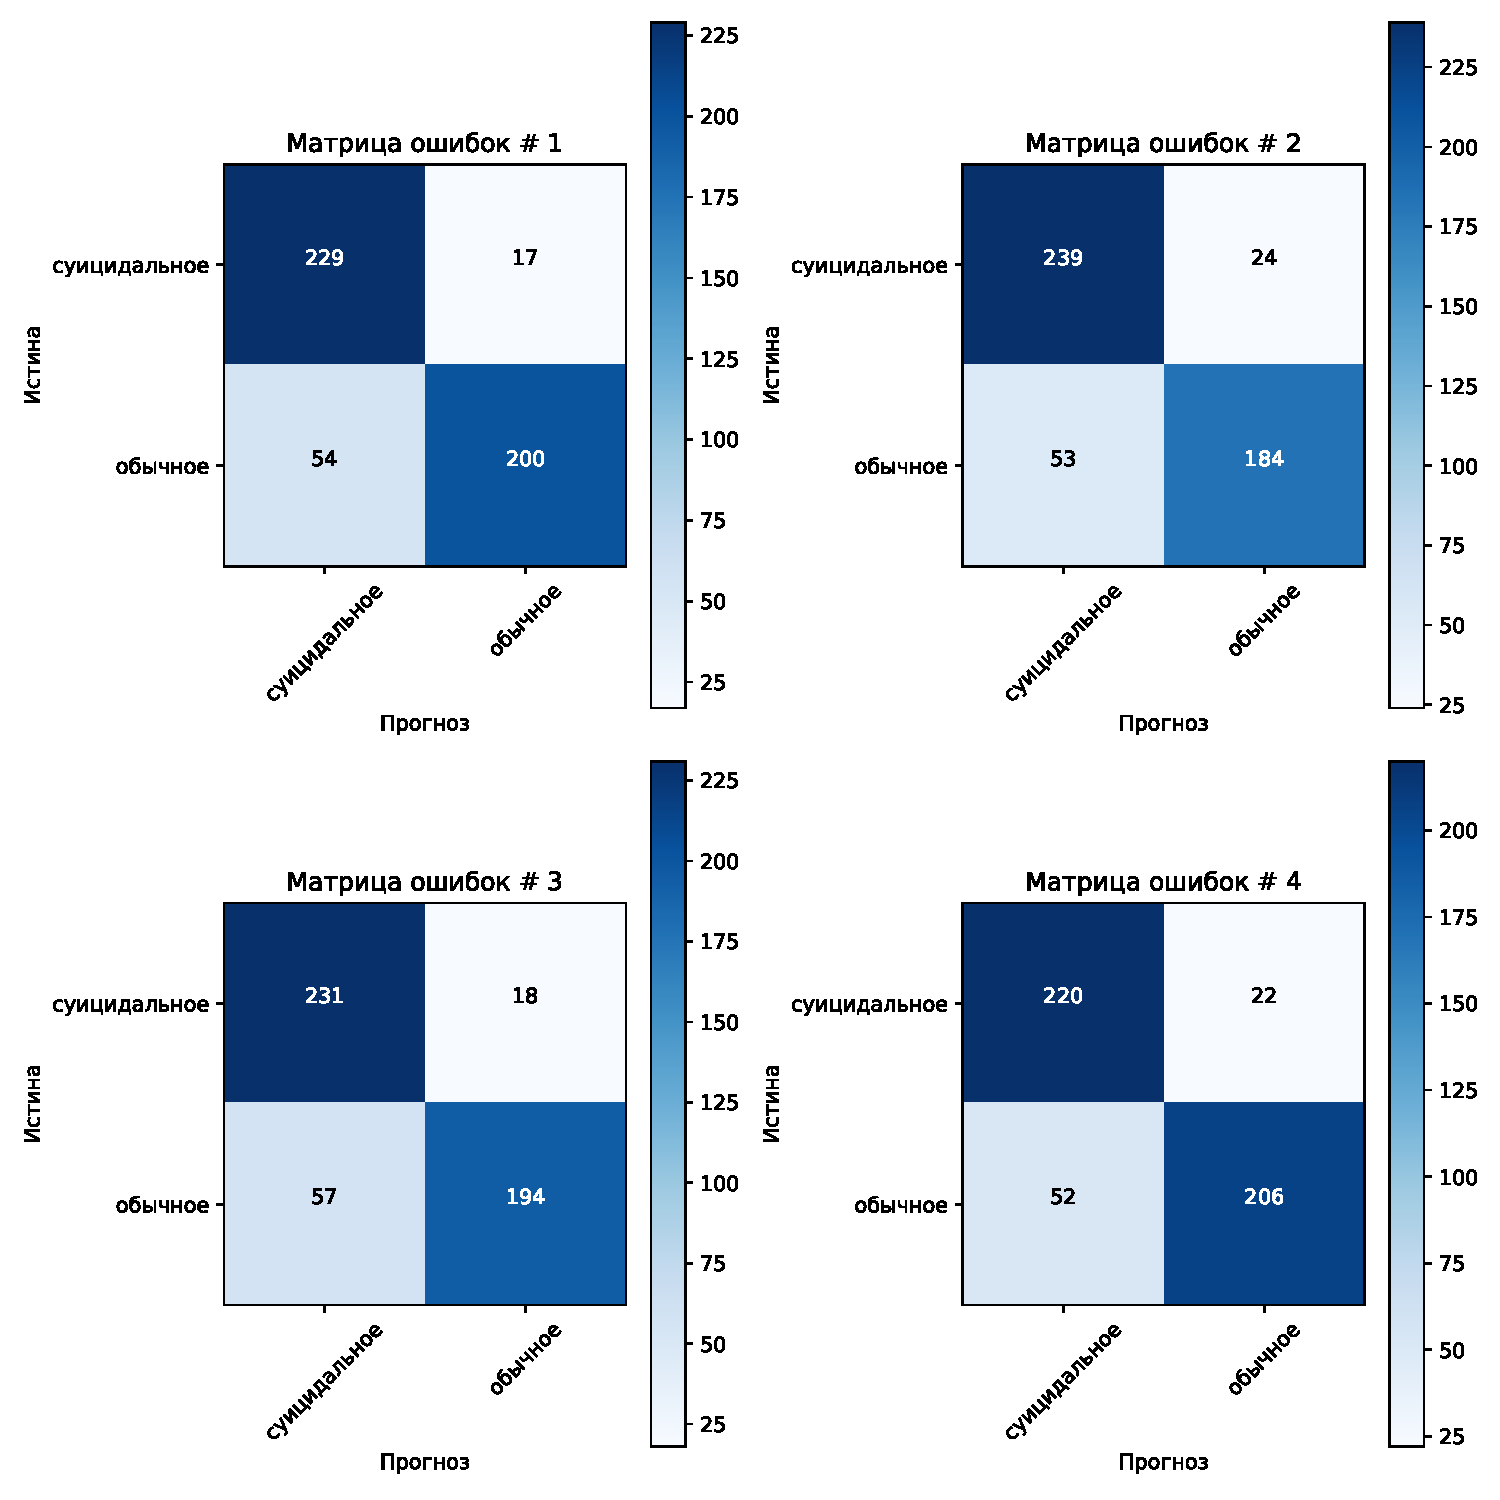
\includegraphics[width=\textwidth]{inc/plots/gradientMatrBag.pdf}
	\caption{ Матрицы ошибок в зависимости от номера разбиения, полученные с использованием градиентного бустинга (метод векторизации -- ``мешок слов''). }
	\label{img:gradientMatrBag}
\end{figure}

На рисунке \ref{img:gradientMetricsBag} представлены оценки классификатора, полученные с использованием градиентного бустинга, метод векторизации -- ``мешок слов''.
\begin{figure}[H]
	\centering
	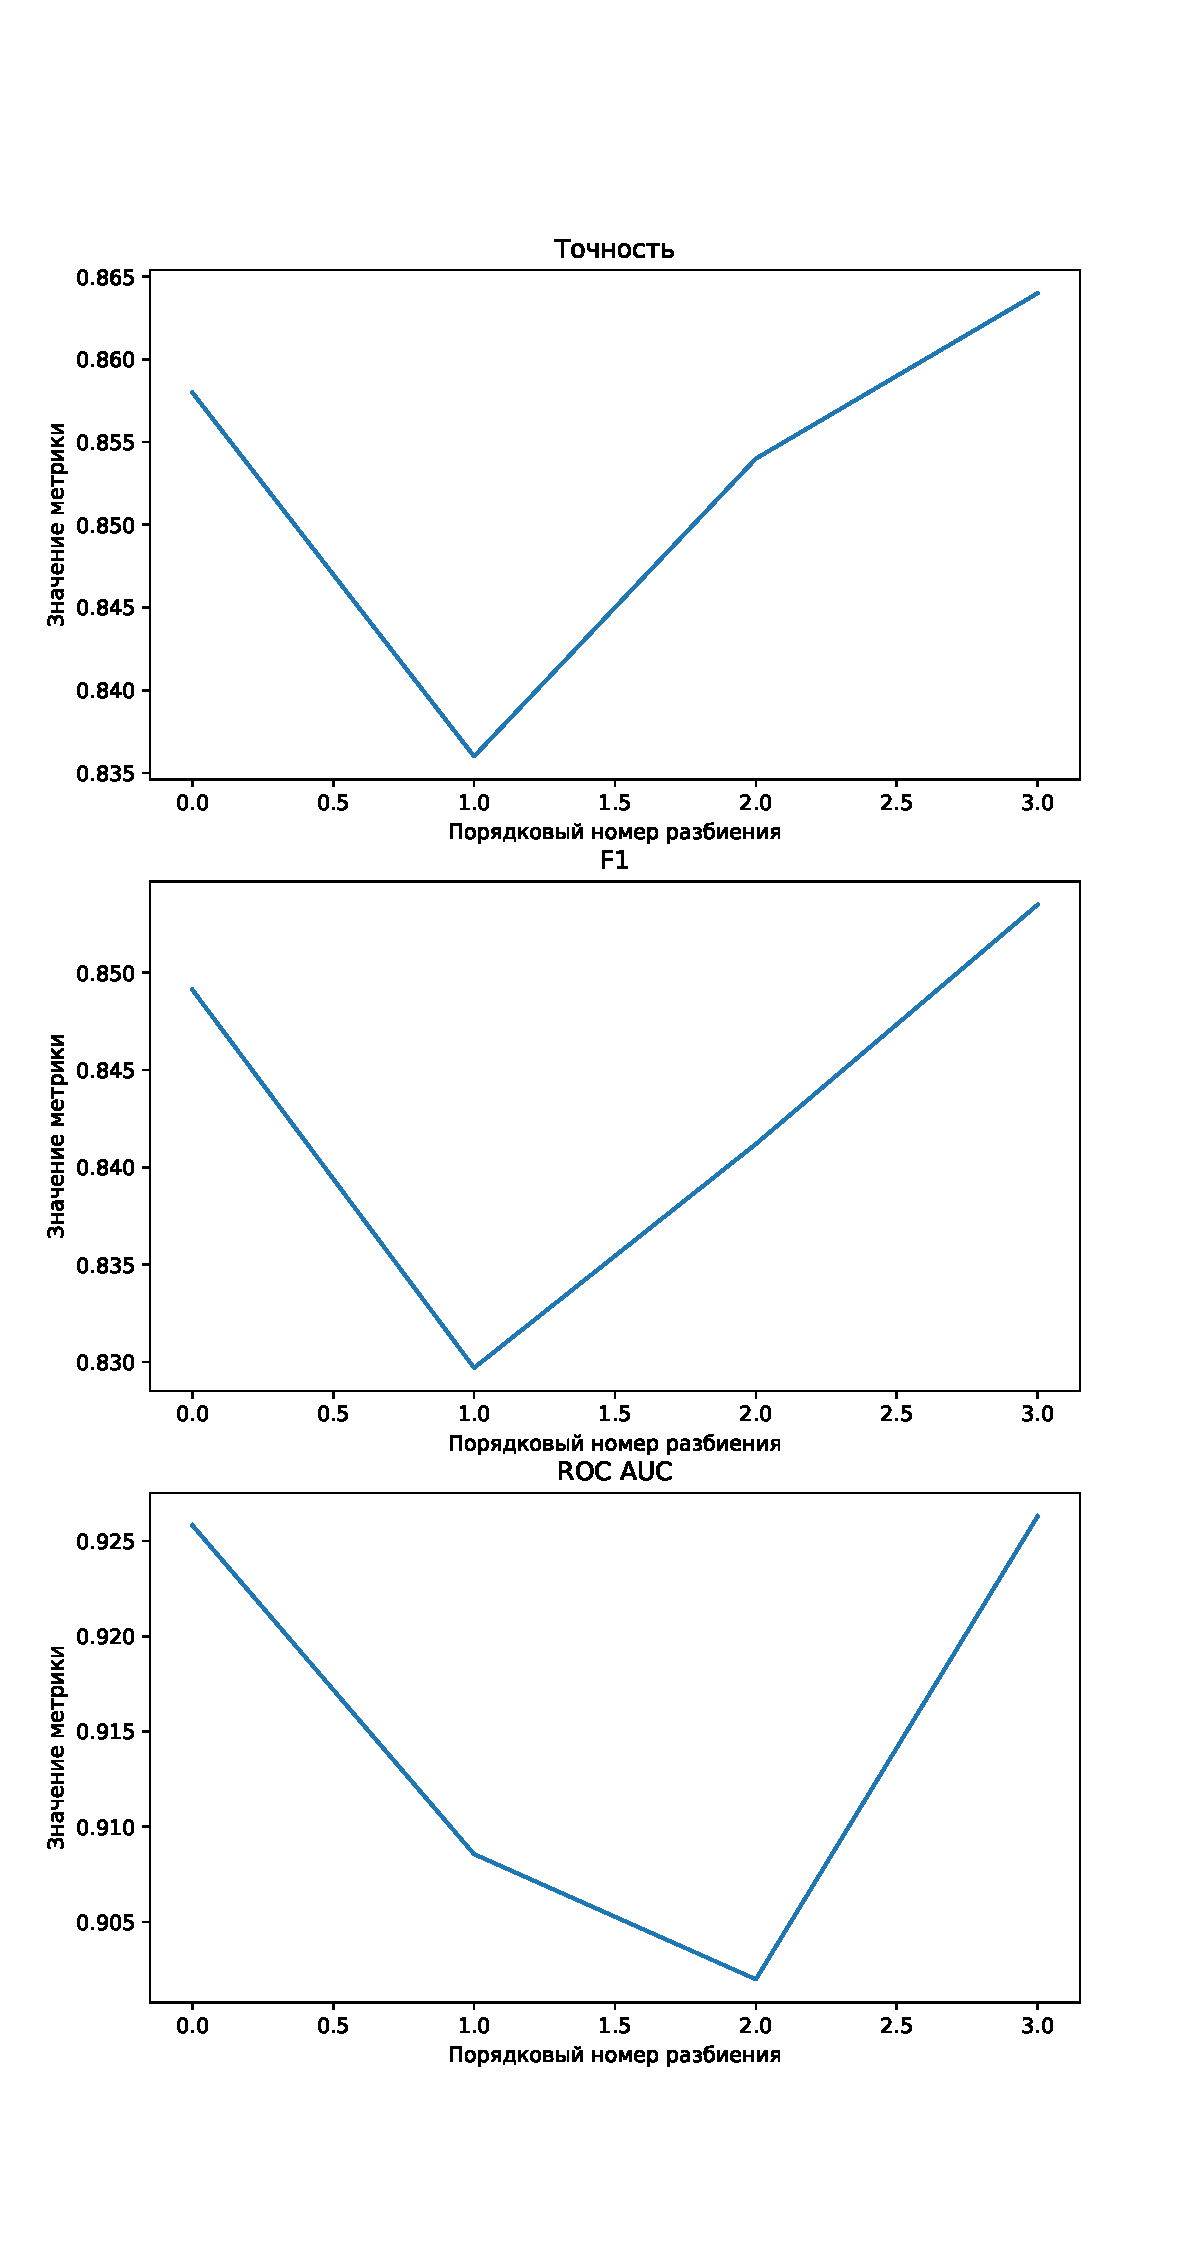
\includegraphics[height=23cm]{inc/plots/gradientMetricsBag.pdf}
	\caption{ Оценки классификатора в зависимости от номера разбиения, полученные с использованием градиентного бустинга (метод векторизации --  ``мешок слов''). }
	\label{img:gradientMetricsBag}
\end{figure}

Параметры модели при применении векторизации BERT:
\begin{itemize}
	\item коэффициент обучения -- 0.3;
	\item количество классификаторов в ансамбле -- 245;
	\item минимальное количество образцов для разбиения узла дерева решений -- 16.
\end{itemize}

На рисунке \ref{img:gradientMatrBert} представлены матрицы ошибок, полученные с использованием градиентного бустинга, метод векторизации -- BERT.
\begin{figure}[H]
	\centering
	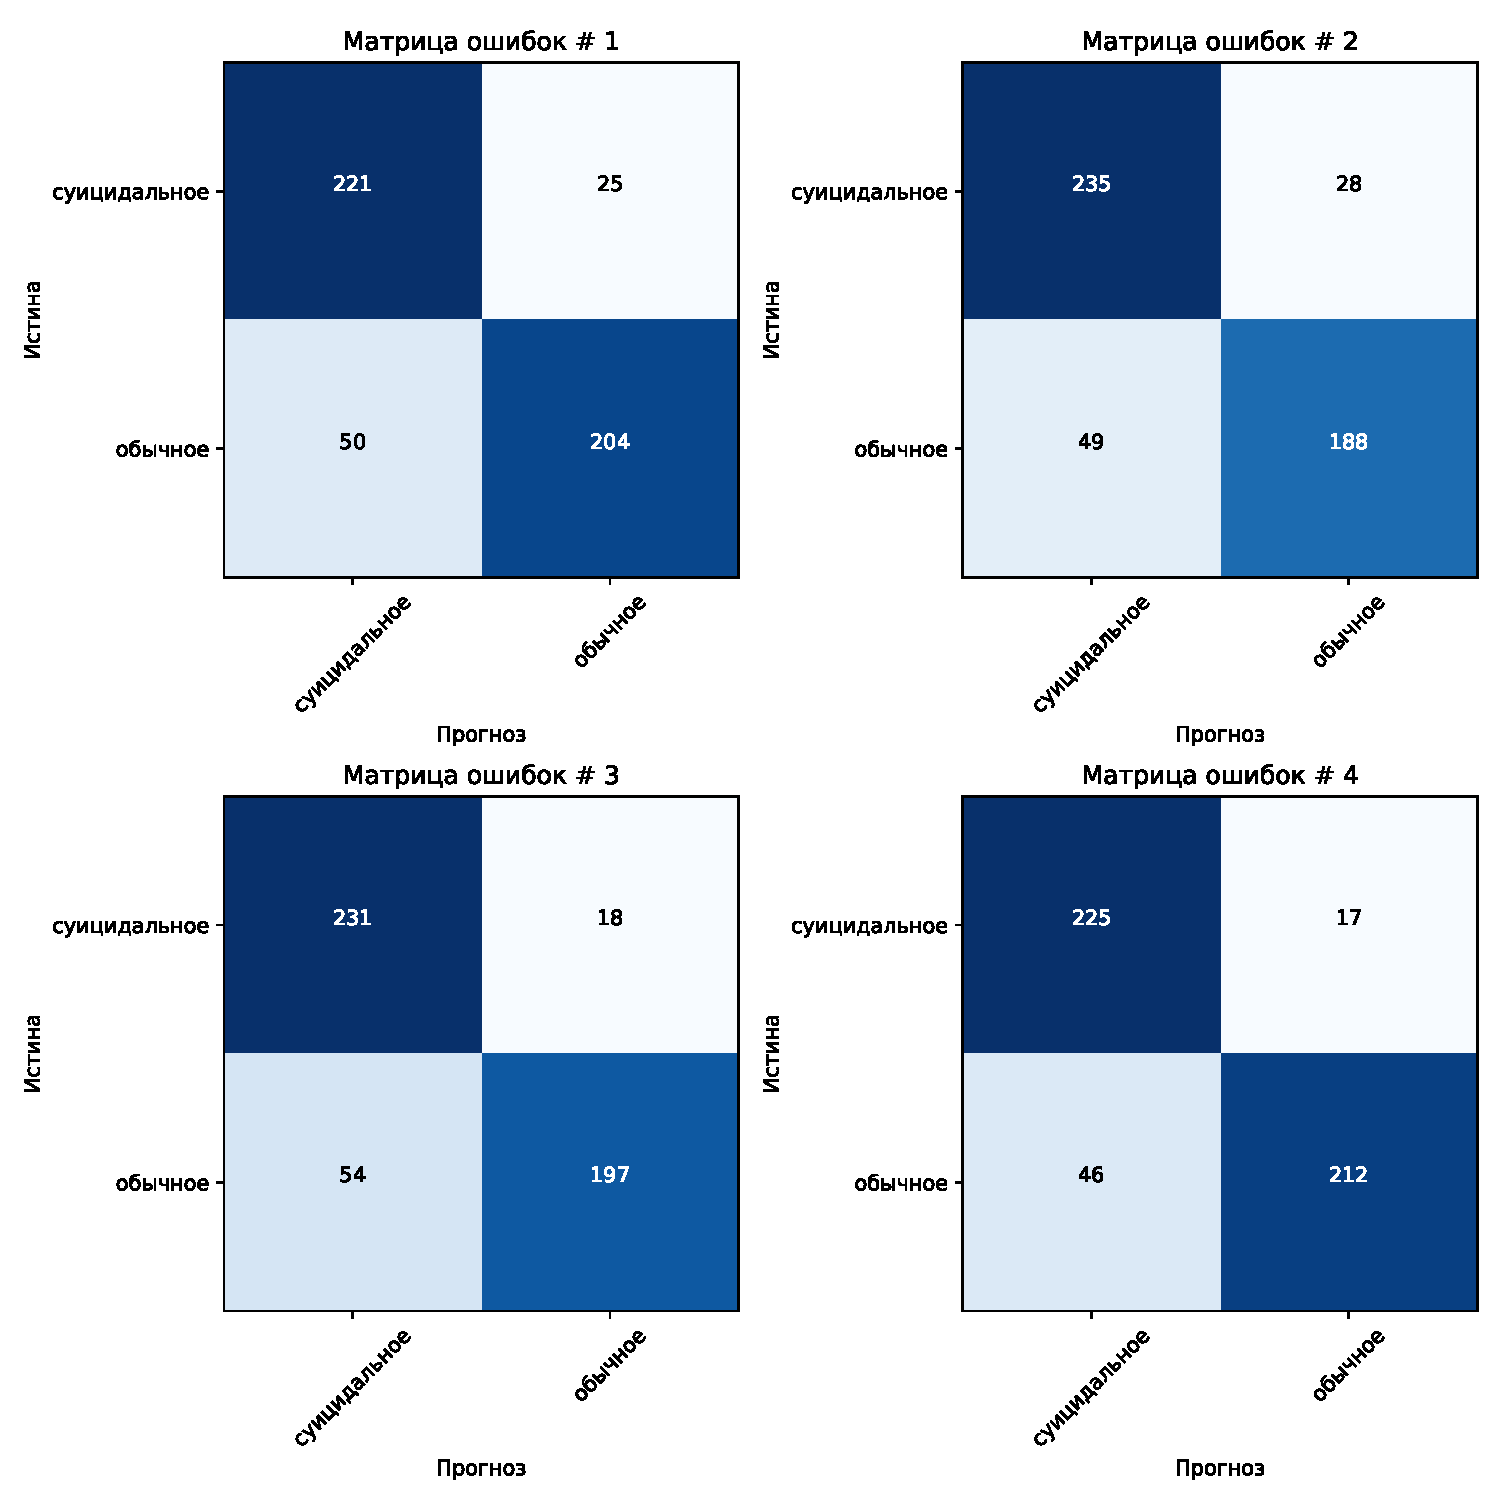
\includegraphics[width=\textwidth]{inc/plots/gradientMatrBert.pdf}
	\caption{ Матрицы ошибок в зависимости от номера разбиения, полученные с использованием градиентного бустинга (метод векторизации -- BERT). }
	\label{img:gradientMatrBert}
\end{figure}

На рисунке \ref{img:gradientMetricsBert} представлены оценки классификатора, полученные с использованием градиентного бустинга, метод векторизации -- BERT.
\begin{figure}[H]
	\centering
	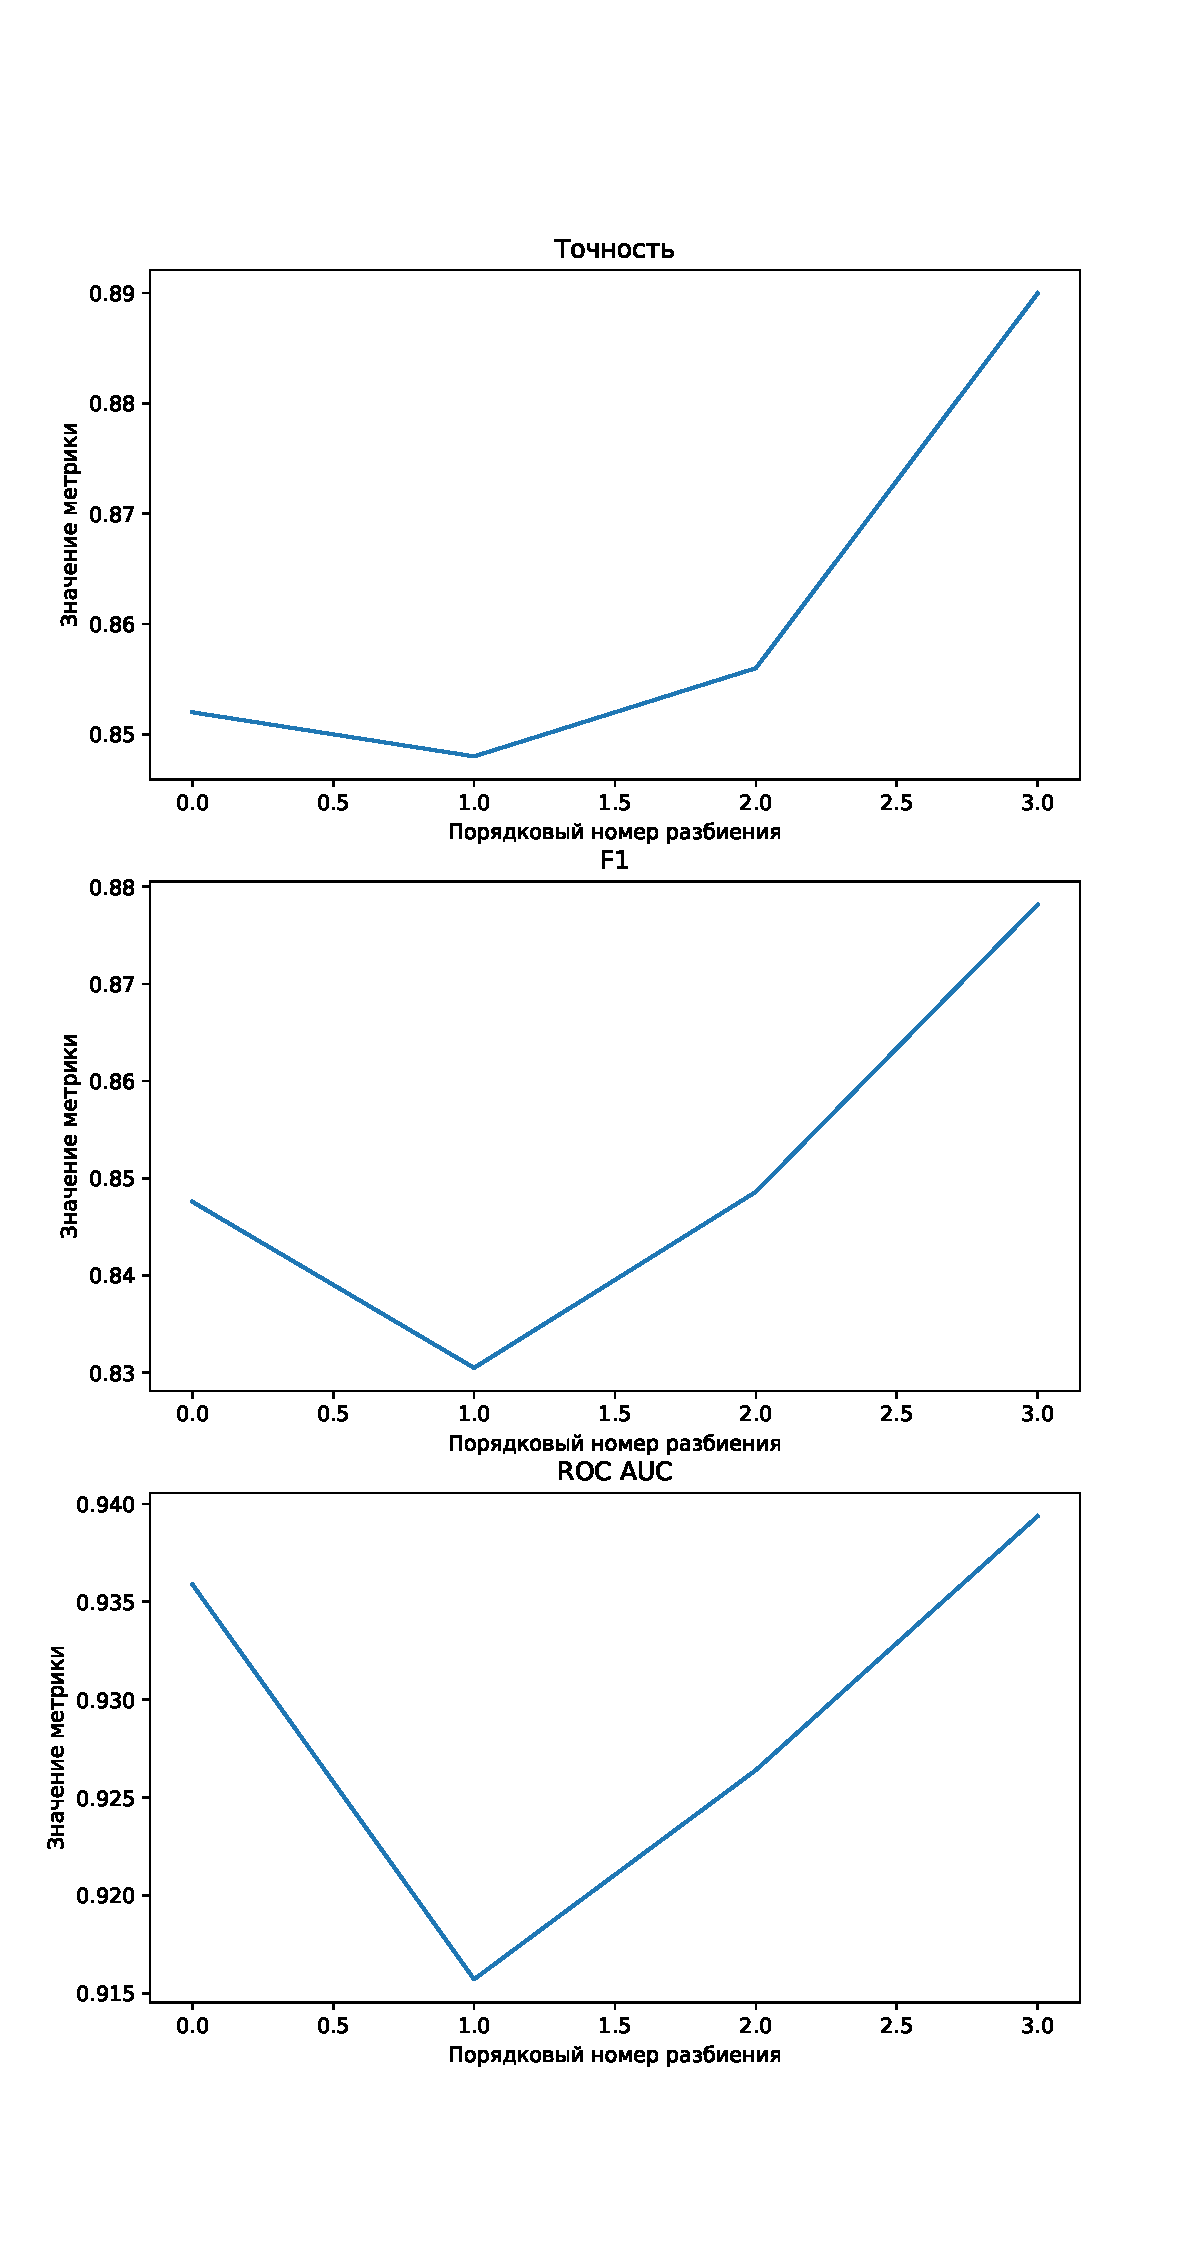
\includegraphics[height=23cm]{inc/plots/gradientMetricsBert.pdf}
	\caption{ Оценки классификатора в зависимости от номера разбиения, полученные с использованием градиентного бустинга (метод векторизации -- BERT). }
	\label{img:gradientMetricsBert}
\end{figure}



\subsection{Метод случайного леса }

Параметры модели при применении метода векторизации ``мешок слов'':
\begin{itemize}
	\item максимальная глубина -- определяет максимальную глубину дерева решений -- 300;
	\item максимальное количество признаков -- определяет максимальное количество признаков, используемых для разбиения узла дерева решений, может принимать значение функции -- $log_2$;
	\item количество классификаторов в ансамбле -- определяет количество деревьев, используемых в алгоритме, -- 850.
\end{itemize}

На рисунке \ref{img:randomMatrBag} представлены матрицы ошибок, полученные с использованием метода случайного леса, метод векторизации -- ``мешок слов''.
\begin{figure}[H]
	\centering
	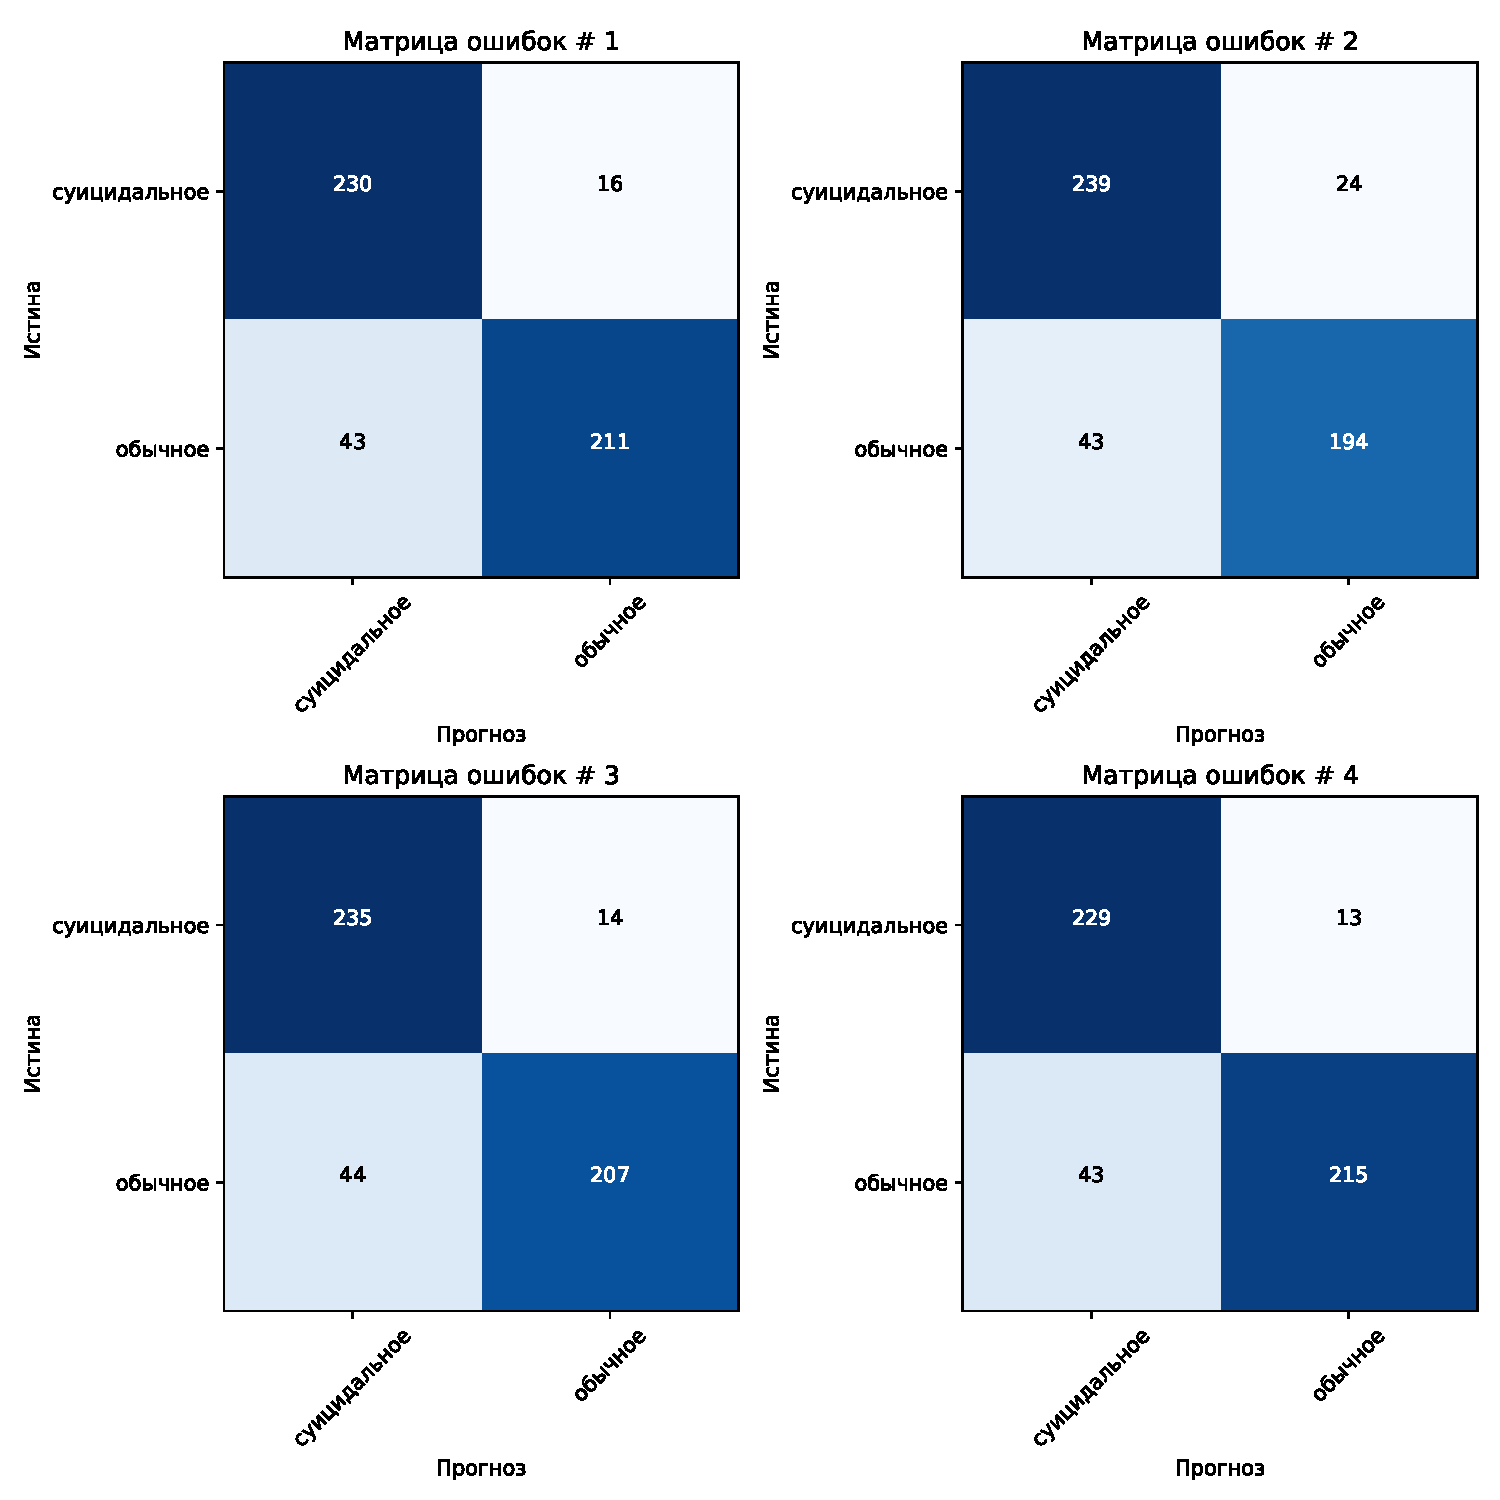
\includegraphics[width=\textwidth]{inc/plots/randomMatrBag.pdf}
	\caption{ Матрицы ошибок в зависимости от номера разбиения, полученные с использованием метода случайного леса (метод векторизации -- ``мешок слов''). }
	\label{img:randomMatrBag}
\end{figure}

На рисунке \ref{img:randomMetricsBag} представлены оценки классификатора, полученные с использованием метода случайного леса, метод векторизации -- ``мешок слов''.
\begin{figure}[H]
	\centering
	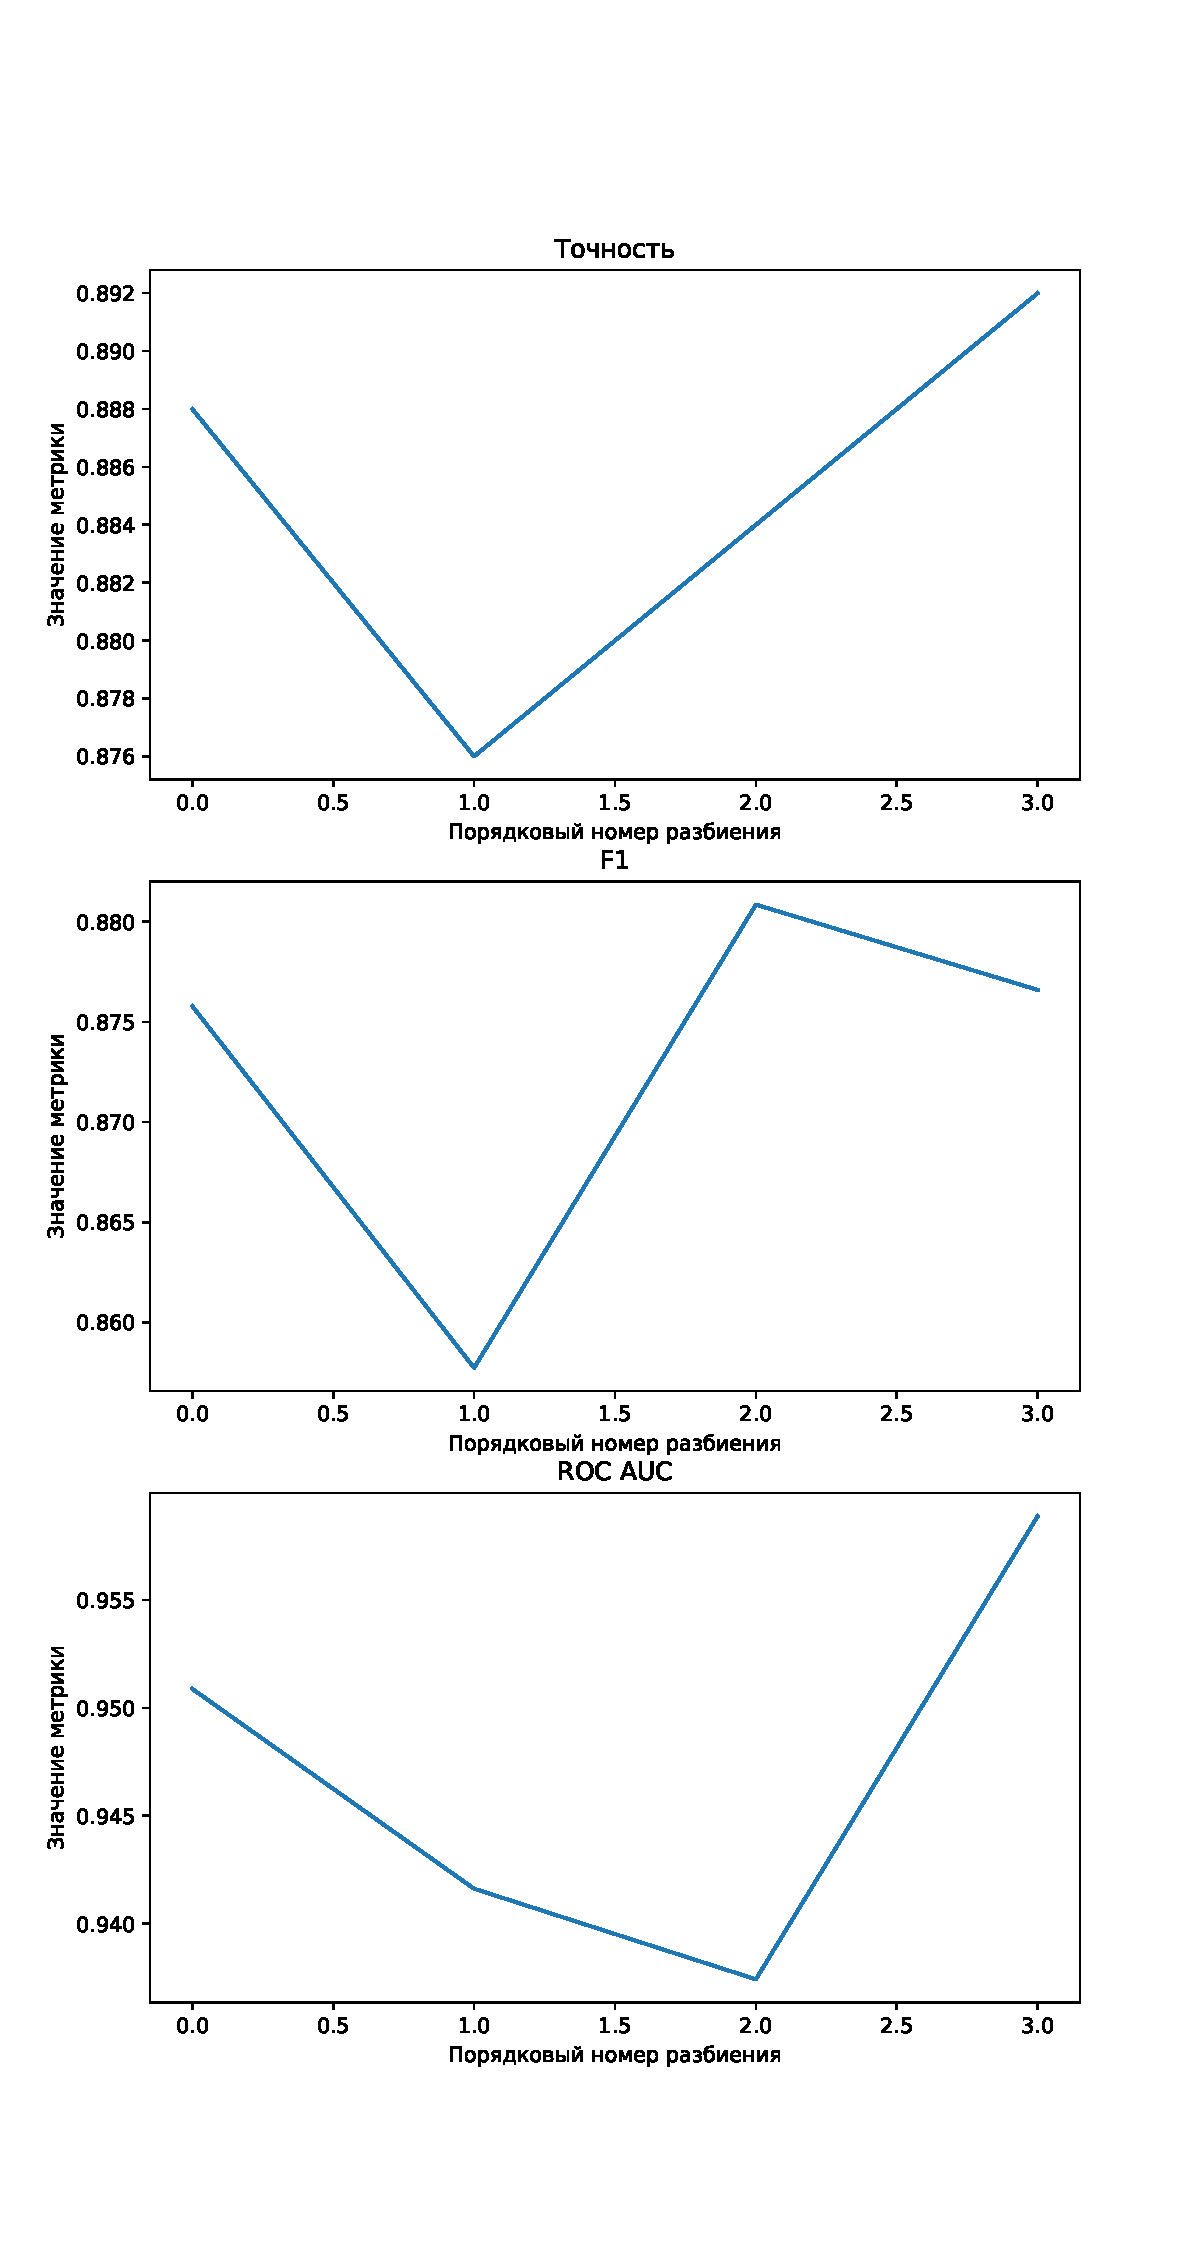
\includegraphics[height=23cm]{inc/plots/randomMetricsBag.pdf}
	\caption{ Оценки классификатора в зависимости от номера разбиения, полученные с использованием метода случайного леса (метод векторизации --  ``мешок слов''). }
	\label{img:randomMetricsBag}
\end{figure}


Параметры модели при применении векторизации BERT:
\begin{itemize}
	\item максимальная глубина -- отсутствует;
	\item максимальное количество признаков -- $log_2$;
	\item количество классификаторов в ансамбле -- 2600.
\end{itemize}

На рисунке \ref{img:randomMatrBert} представлены матрицы ошибок, полученные с использованием метода случайного леса, метод векторизации -- BERT.
\begin{figure}[H]
	\centering
	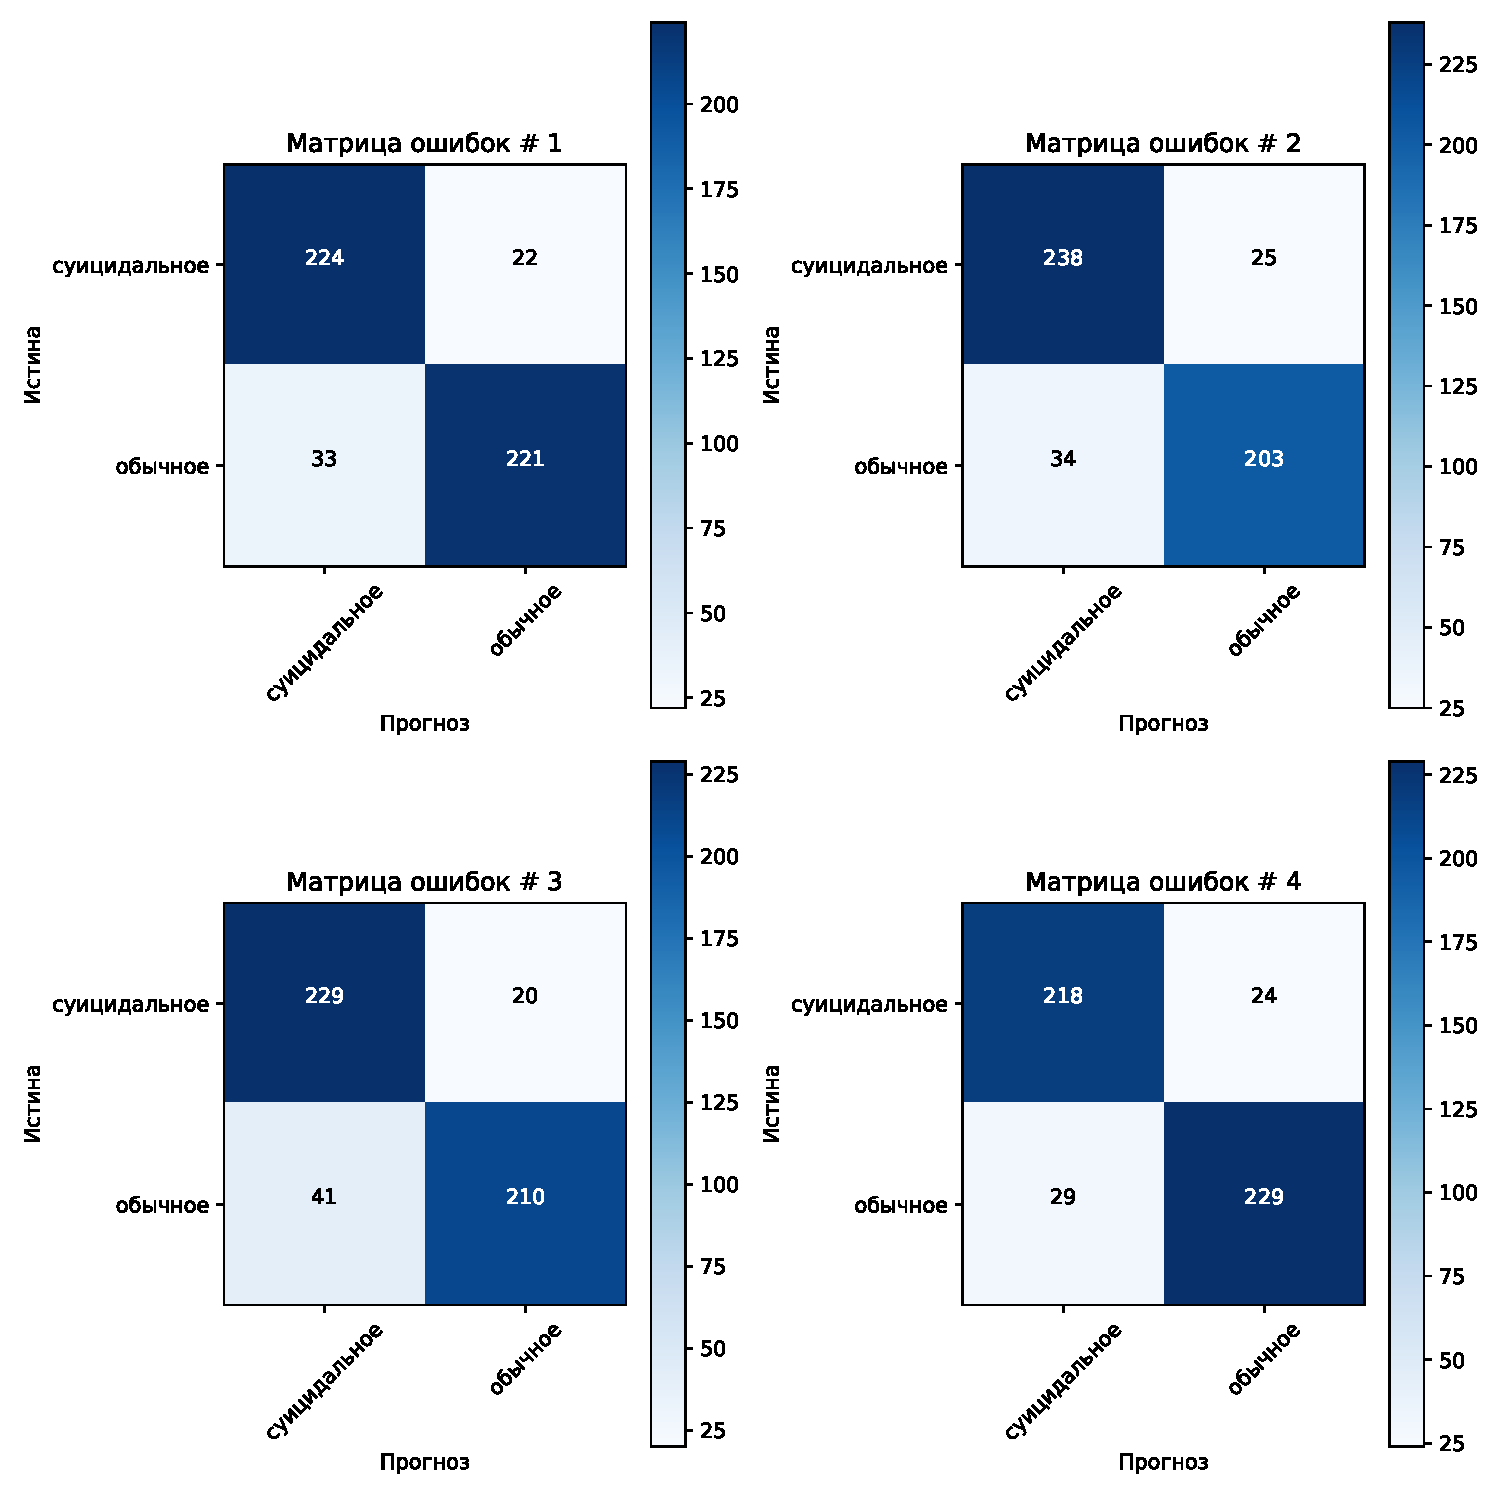
\includegraphics[width=\textwidth]{inc/plots/randomMatrBert.pdf}
	\caption{ Матрицы ошибок в зависимости от номера разбиения, полученные с использованием метода случайного леса (метод векторизации -- BERT). }
	\label{img:randomMatrBert}
\end{figure}

На рисунке \ref{img:randomMetricsBert} представлены оценки классификатора, полученные с использованием метода случайного леса, метод векторизации -- BERT.
\begin{figure}[H]
	\centering
	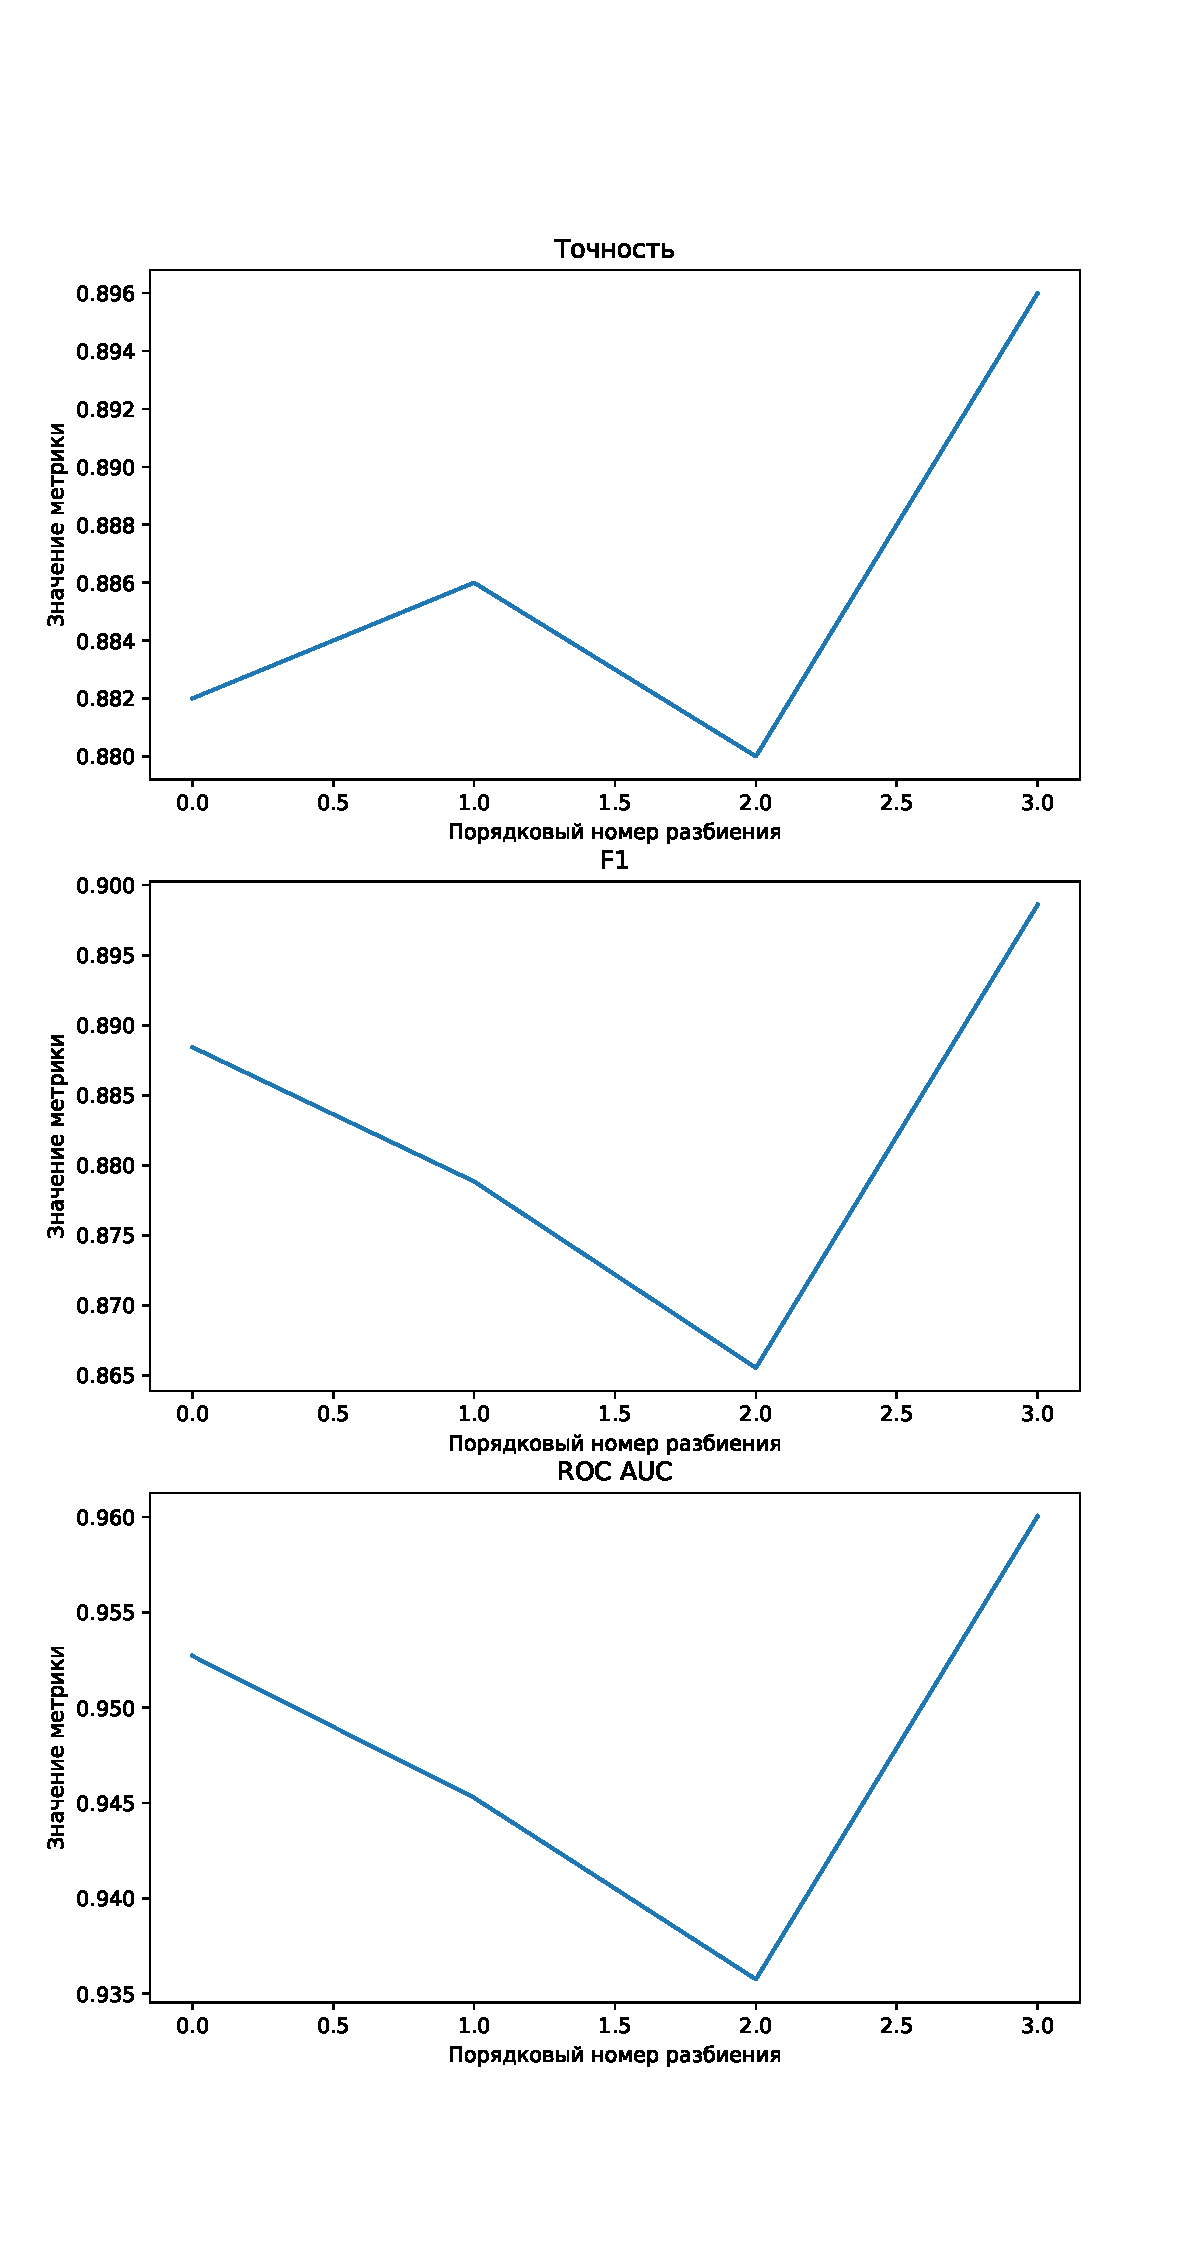
\includegraphics[height=23cm]{inc/plots/randomMetricsBert.pdf}
	\caption{ Оценки классификатора в зависимости от номера разбиения, полученные с использованием метода случайного леса (метод векторизации -- BERT). }
	\label{img:randomMetricsBert}
\end{figure}



\subsection{Метод опорных векторов }

Параметры модели при применении метода векторизации ``мешок слов'':
\begin{itemize}
	\item регуляризационный параметр -- определяет степень регуляризации модели -- 7.0;
	\item ядро -- определяет тип ядра, используемого в модели -- RBF (радиальное базисной функции);
	\item коэффициент ядра -- определяет ``ширину'' ядра -- значение вычисляется как обратная величина произведения количества признаков на дисперсию признаков.
\end{itemize}

На рисунке \ref{img:svcMatrBag} представлены матрицы ошибок, полученные с использованием метода опорных векторов, метод векторизации -- ``мешок слов''.
\begin{figure}[H]
	\centering
	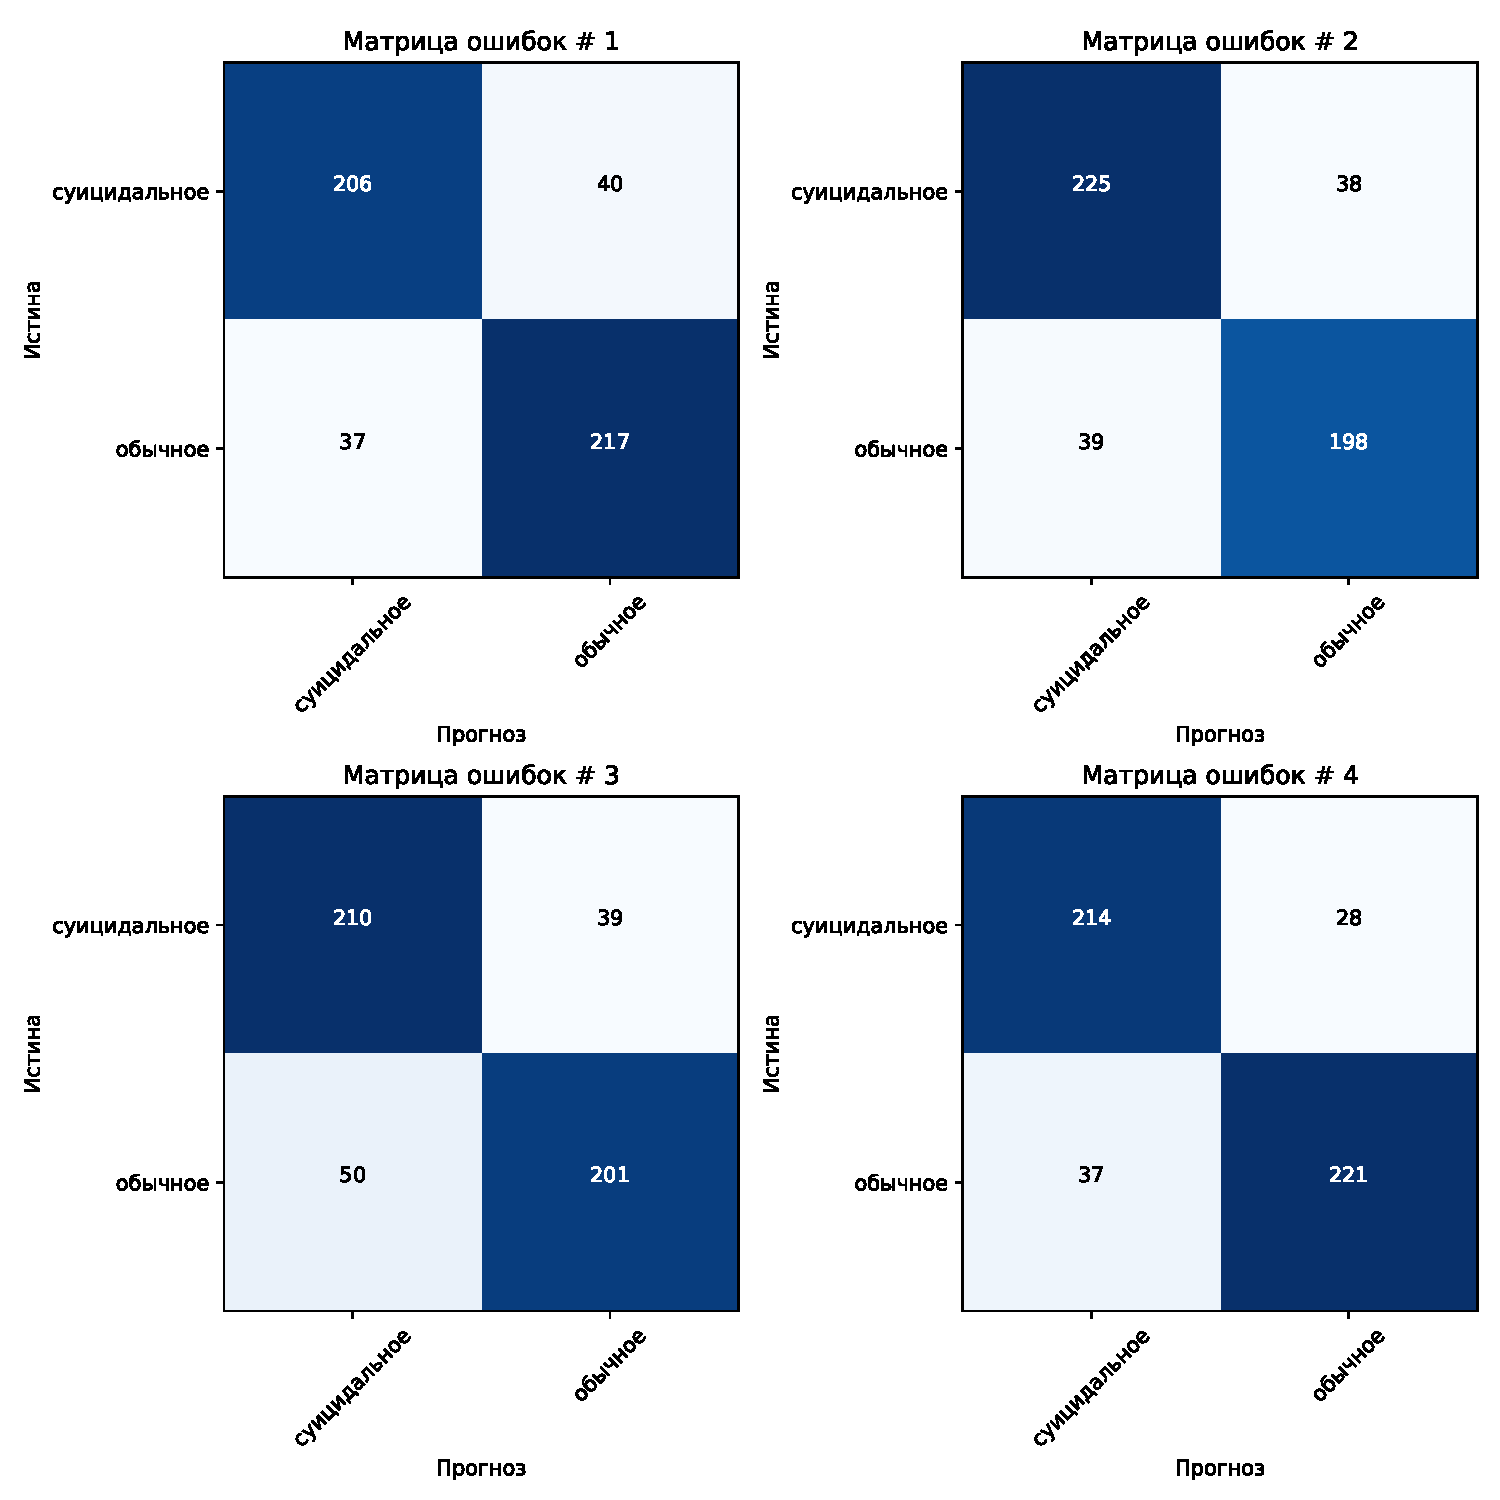
\includegraphics[width=\textwidth]{inc/plots/svcMatrBag.pdf}
	\caption{ Матрицы ошибок в зависимости от номера разбиения, полученные с использованием метода опорных векторов (метод векторизации -- ``мешок слов''). }
	\label{img:svcMatrBag}
\end{figure}

На рисунке \ref{img:svcMetricsBag} представлены оценки классификатора, полученные с использованием метода опорных векторов, метод векторизации -- ``мешок слов''.
\begin{figure}[H]
	\centering
	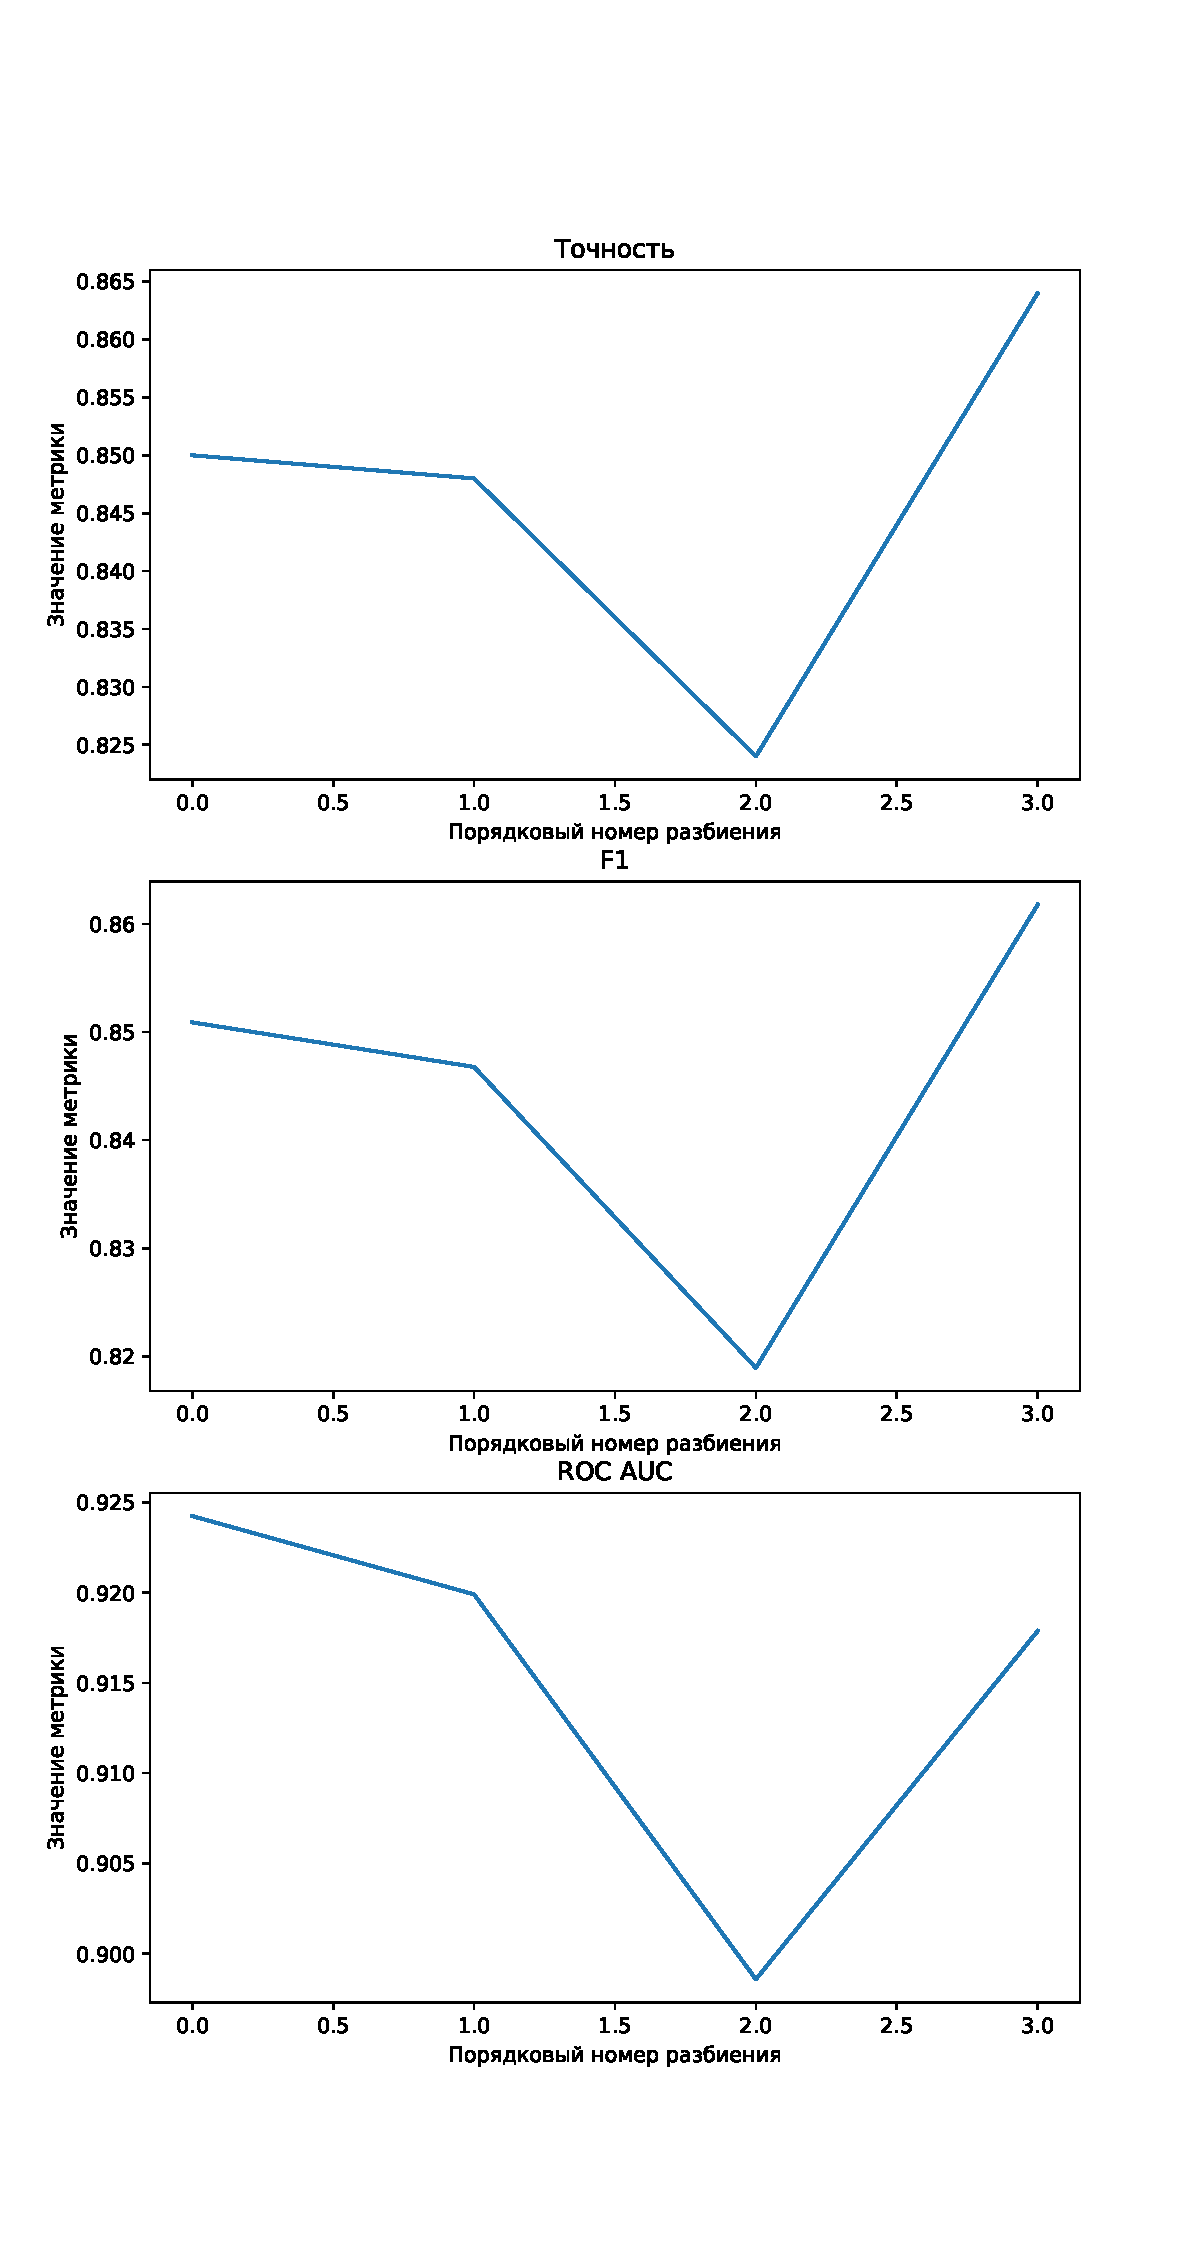
\includegraphics[height=23cm]{inc/plots/svcMetricsBag.pdf}
	\caption{ Оценки классификатора в зависимости от номера разбиения, полученные с использованием метода опорных векторов (метод векторизации --  ``мешок слов''). }
	\label{img:svcMetricsBag}
\end{figure}


Параметры модели при применении векторизации BERT:
\begin{itemize}
	\item регуляризационный параметр -- 1.5;
	\item ядро -- линейное;
	\item коэффициент ядра -- значение вычисляется как обратная величина произведения количества признаков на дисперсию признаков.
\end{itemize}

На рисунке \ref{img:svcMatrBert} представлены матрицы ошибок, полученные с использованием метода опорных векторов, метод векторизации -- BERT.
\begin{figure}[H]
	\centering
	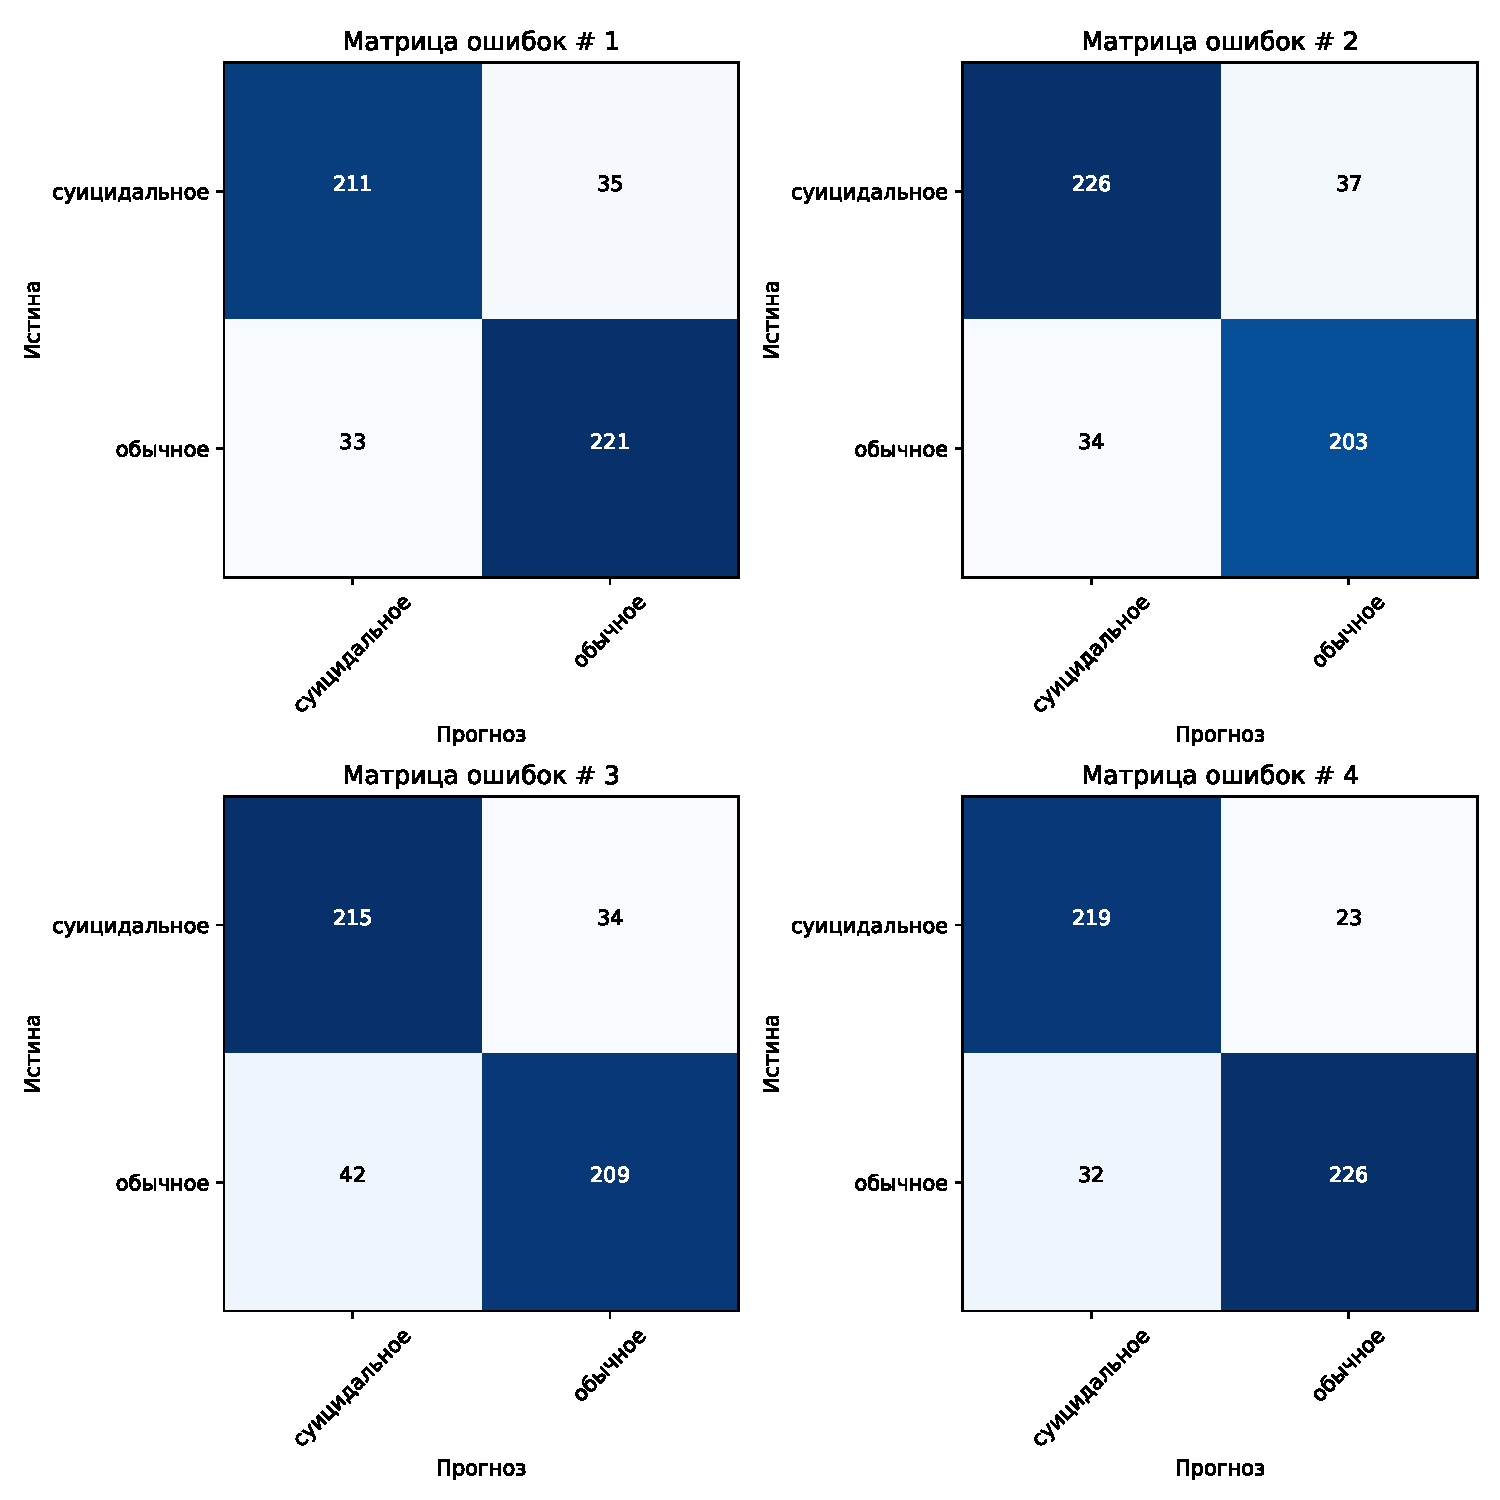
\includegraphics[width=\textwidth]{inc/plots/svcMatrBert.pdf}
	\caption{ Матрицы ошибок в зависимости от номера разбиения, полученные с использованием метода опорных векторов (метод векторизации -- BERT). }
	\label{img:svcMatrBert}
\end{figure}

На рисунке \ref{img:svcMetricsBert} представлены оценки классификатора, полученные с использованием метода опорных векторов, метод векторизации -- BERT.
\begin{figure}[H]
	\centering
	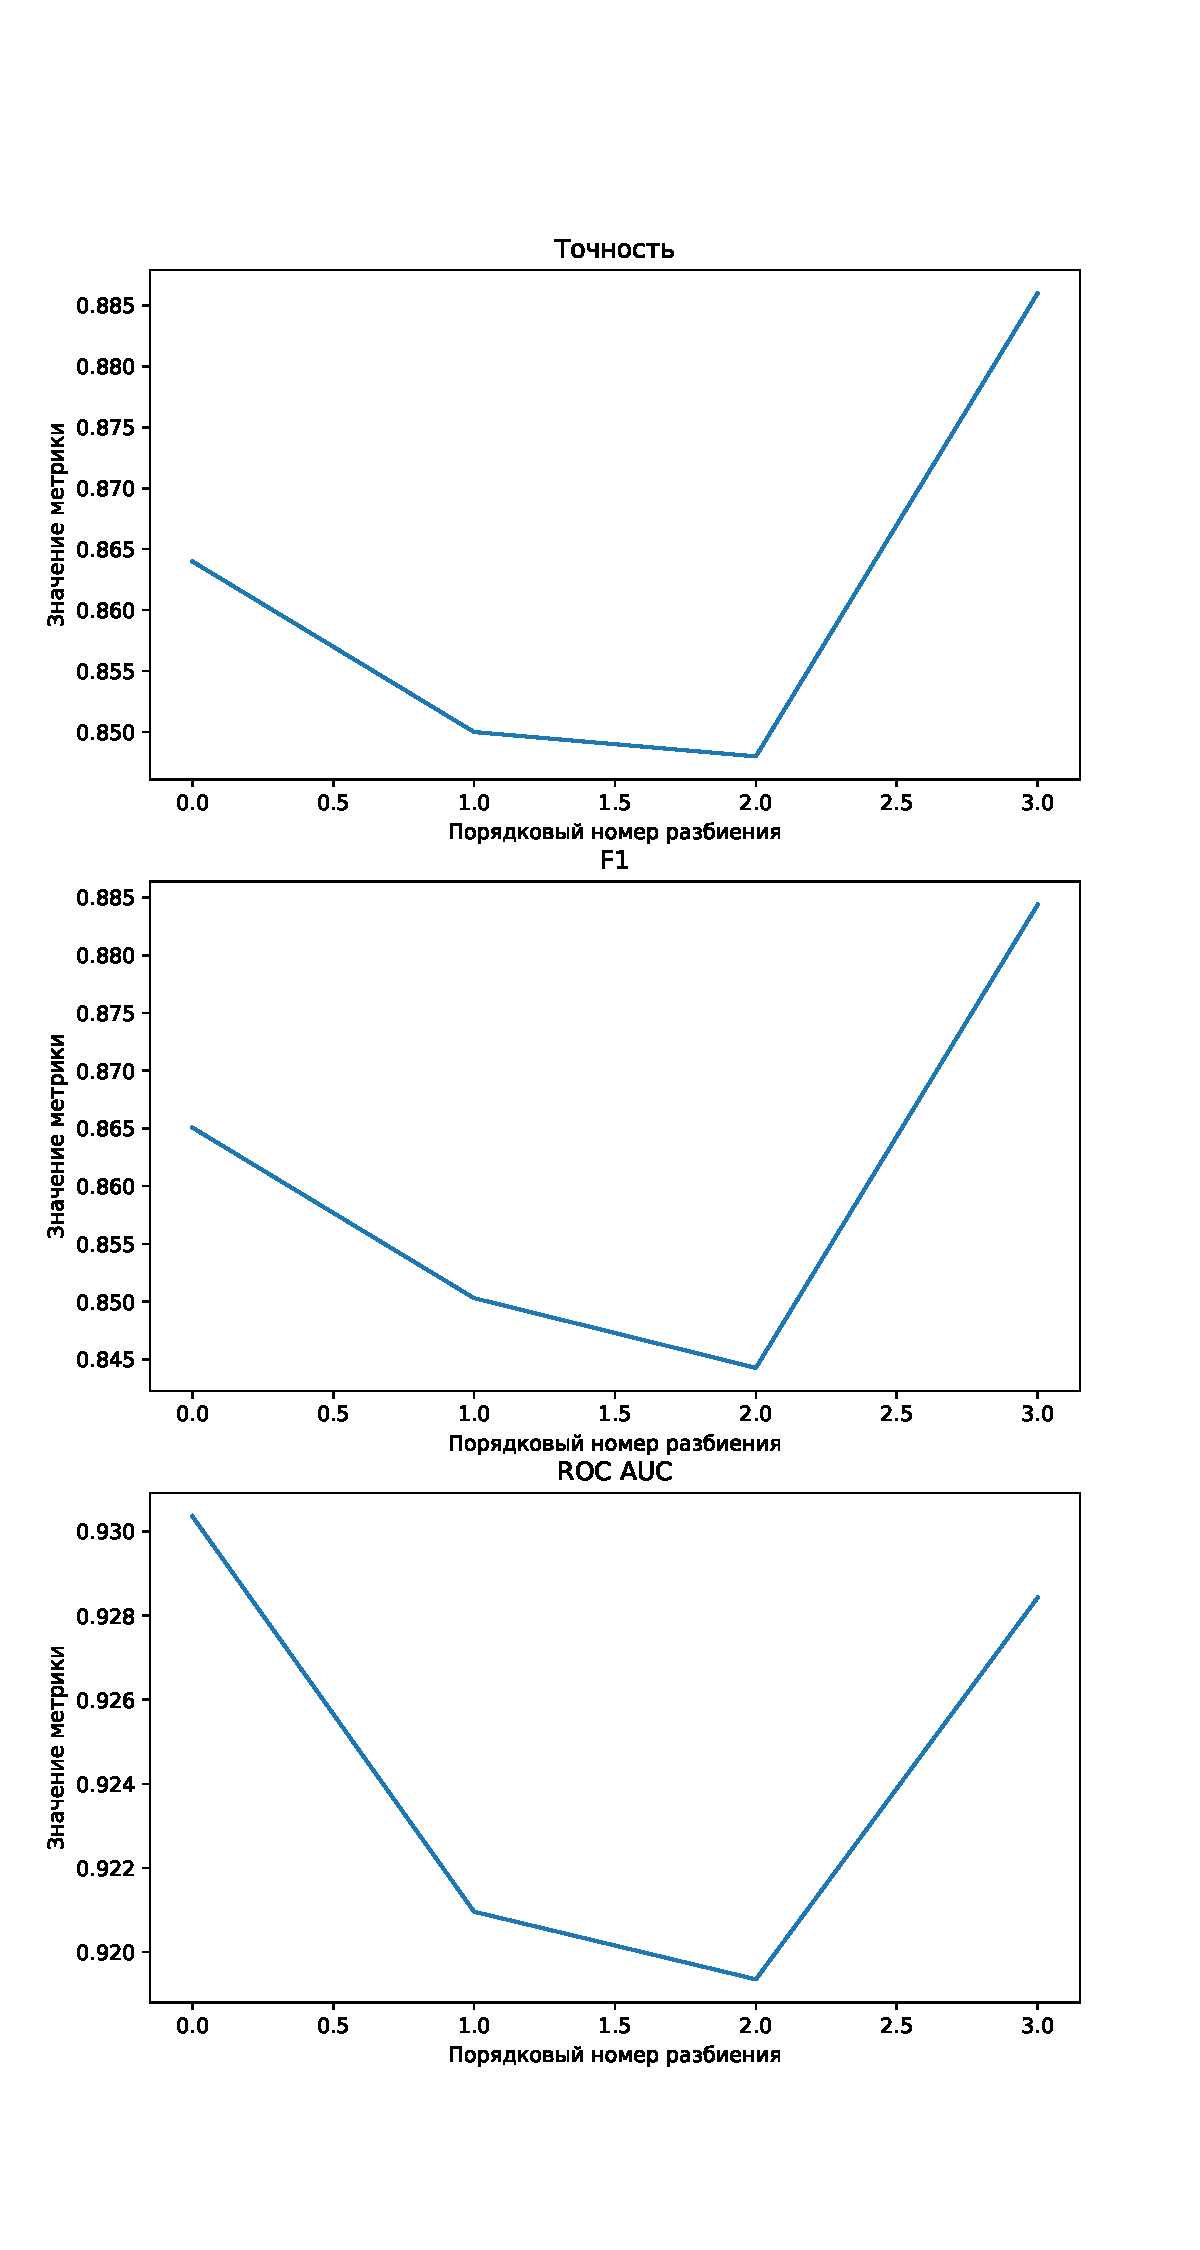
\includegraphics[height=23cm]{inc/plots/svcMetricsBert.pdf}
	\caption{ Оценки классификатора в зависимости от номера разбиения, полученные с использованием метода опорных векторов (метод векторизации -- BERT). }
	\label{img:svcMetricsBert}
\end{figure}



\subsection{Метод K-ближайших соседей }

Параметры модели при применении метода векторизации ``мешок слов'':
\begin{itemize}
	\item количество образцов в листе дерева -- 4;
	\item метрика расстояния -- евклидово расстояние;
	\item количество ближайших соседей -- 5;
	\item метод вычисления весов ближайших соседей -- веса, обратно пропорциональные расстоянию до соседа.
\end{itemize}

На рисунке \ref{img:knnMatrBag} представлены матрицы ошибок, полученные с использованием метода K-ближайших соседей, метод векторизации -- ``мешок слов''.
\begin{figure}[H]
	\centering
	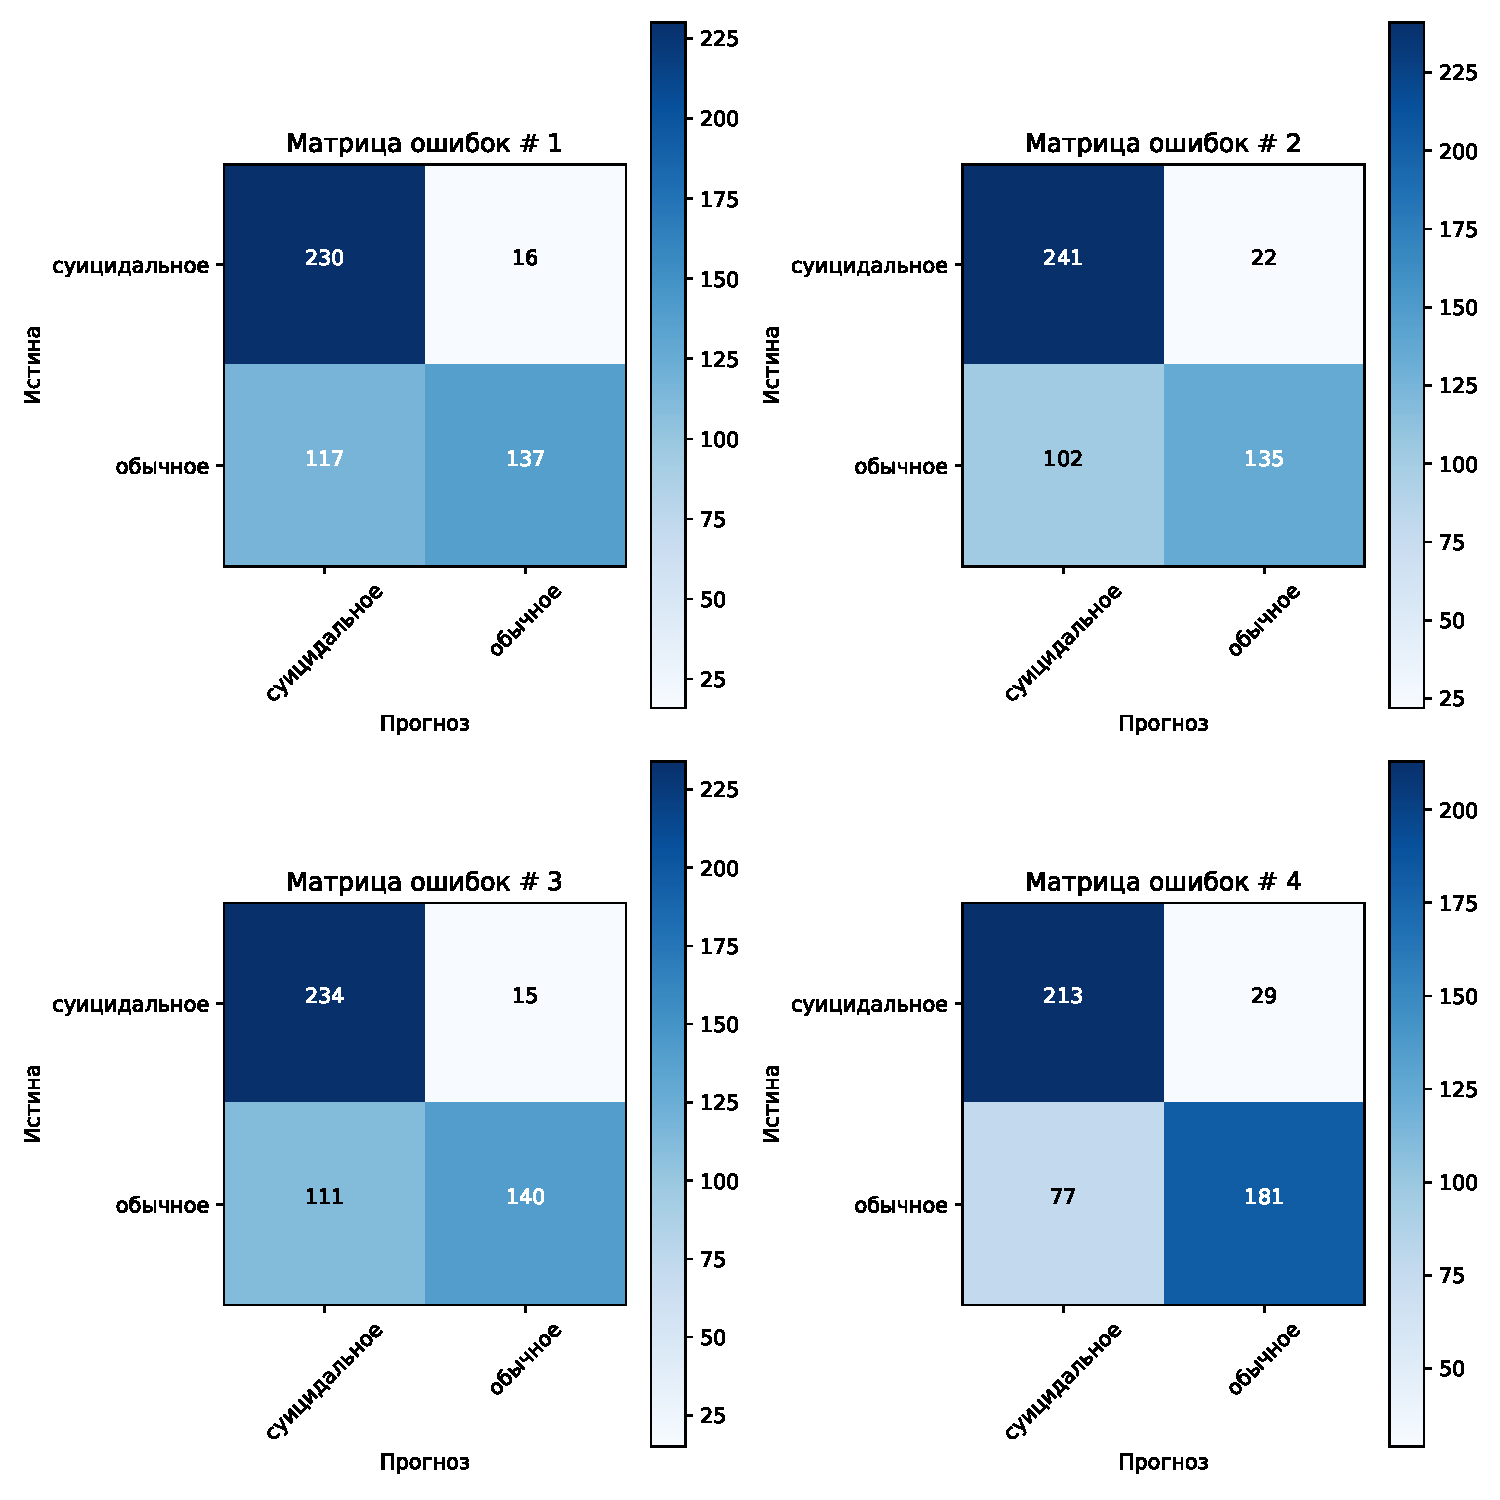
\includegraphics[width=\textwidth]{inc/plots/knnMatrBag.pdf}
	\caption{ Матрицы ошибок в зависимости от номера разбиения, полученные с использованием метода K-ближайших соседей (метод векторизации -- ``мешок слов''). }
	\label{img:knnMatrBag}
\end{figure}

На рисунке \ref{img:knnMetricsBag} представлены оценки классификатора, полученные с использованием метода K-ближайших соседей, метод векторизации -- ``мешок слов''.
\begin{figure}[H]
	\centering
	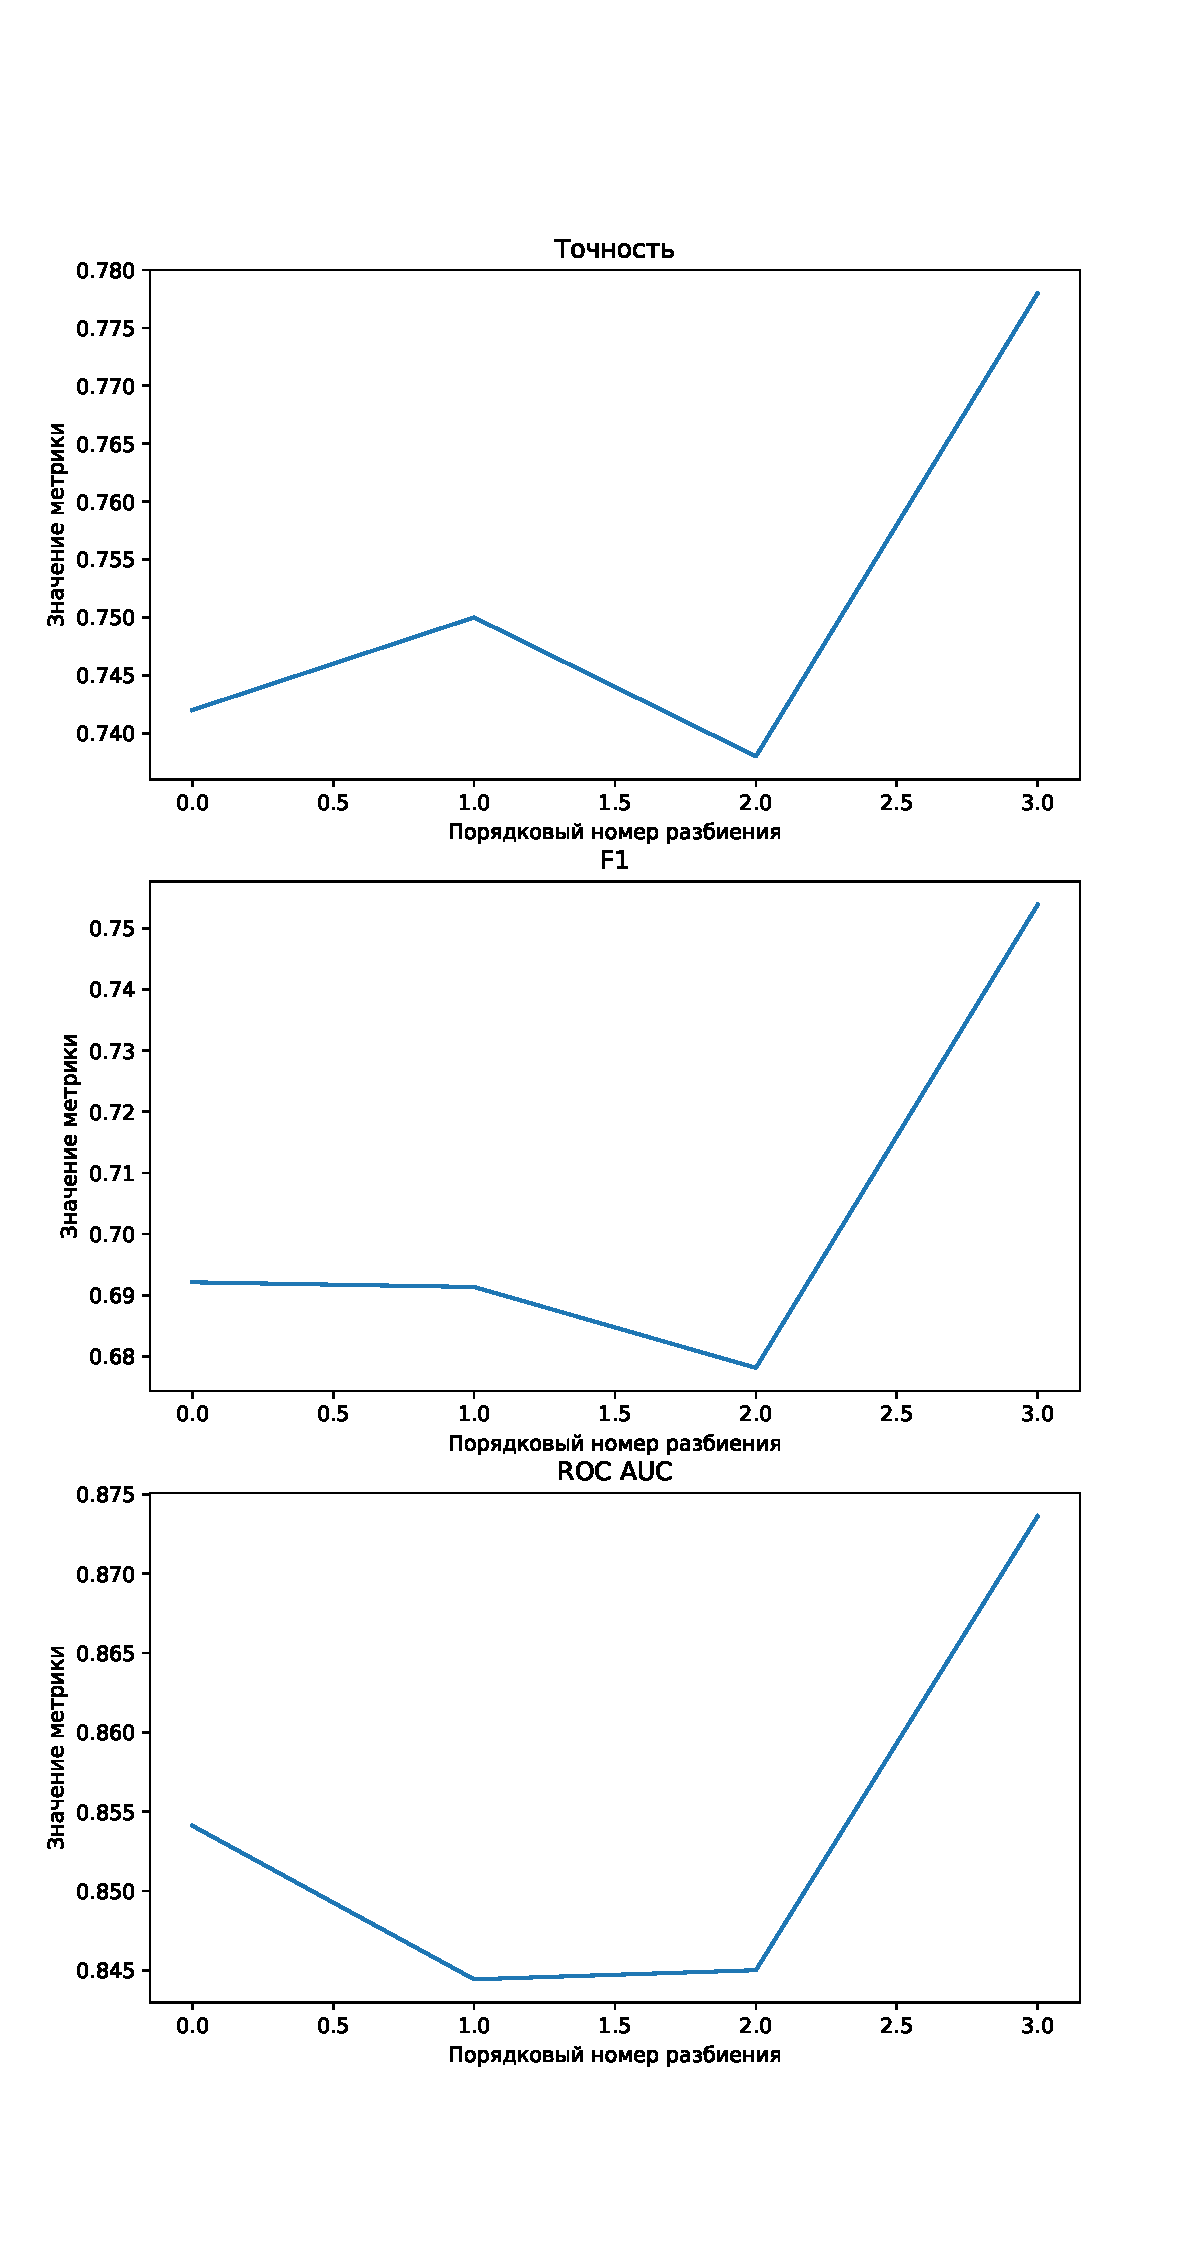
\includegraphics[height=23cm]{inc/plots/knnMetricsBag.pdf}
	\caption{ Оценки классификатора в зависимости от номера разбиения, полученные с использованием метода K-ближайших соседей (метод векторизации --  ``мешок слов''). }
	\label{img:knnMetricsBag}
\end{figure}


Параметры модели при применении векторизации BERT:
\begin{itemize}
	\item количество образцов в листе дерева -- 1;
	\item метрика расстояния -- евклидово расстояние;
	\item количество ближайших соседей -- 6;
	\item метод вычисления весов ближайших соседей -- веса, обратно пропорциональные расстоянию до соседа.
\end{itemize}

На рисунке \ref{img:knnMatrBert} представлены матрицы ошибок, полученные с использованием метода K-ближайших соседей, метод векторизации -- BERT.
\begin{figure}[H]
	\centering
	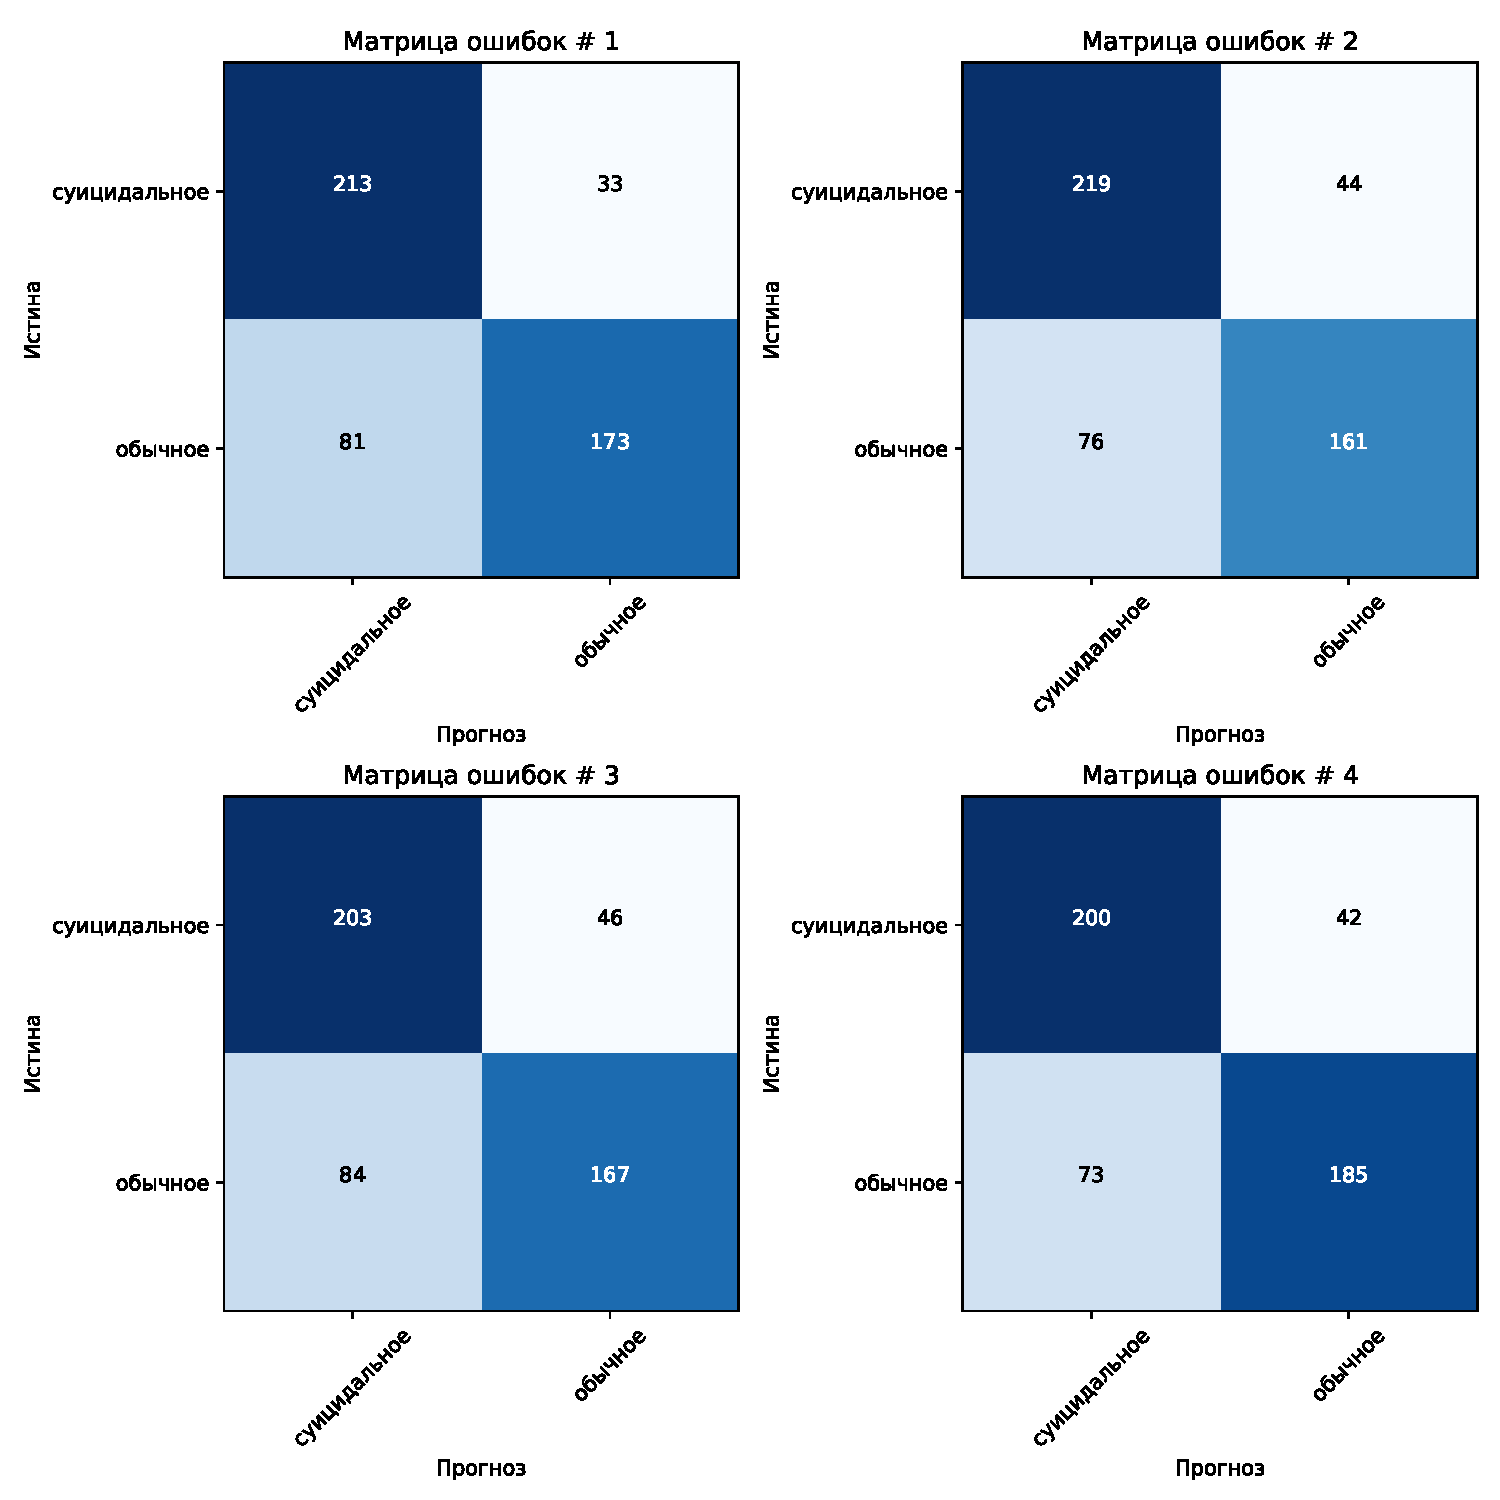
\includegraphics[width=\textwidth]{inc/plots/knnMatrBert.pdf}
	\caption{ Матрицы ошибок в зависимости от номера разбиения, полученные с использованием метода K-ближайших соседей (метод векторизации -- BERT). }
	\label{img:knnMatrBert}
\end{figure}

На рисунке \ref{img:knnMetricsBert} представлены оценки классификатора, полученные с использованием метода K-ближайших соседей, метод векторизации -- BERT.
\begin{figure}[H]
	\centering
	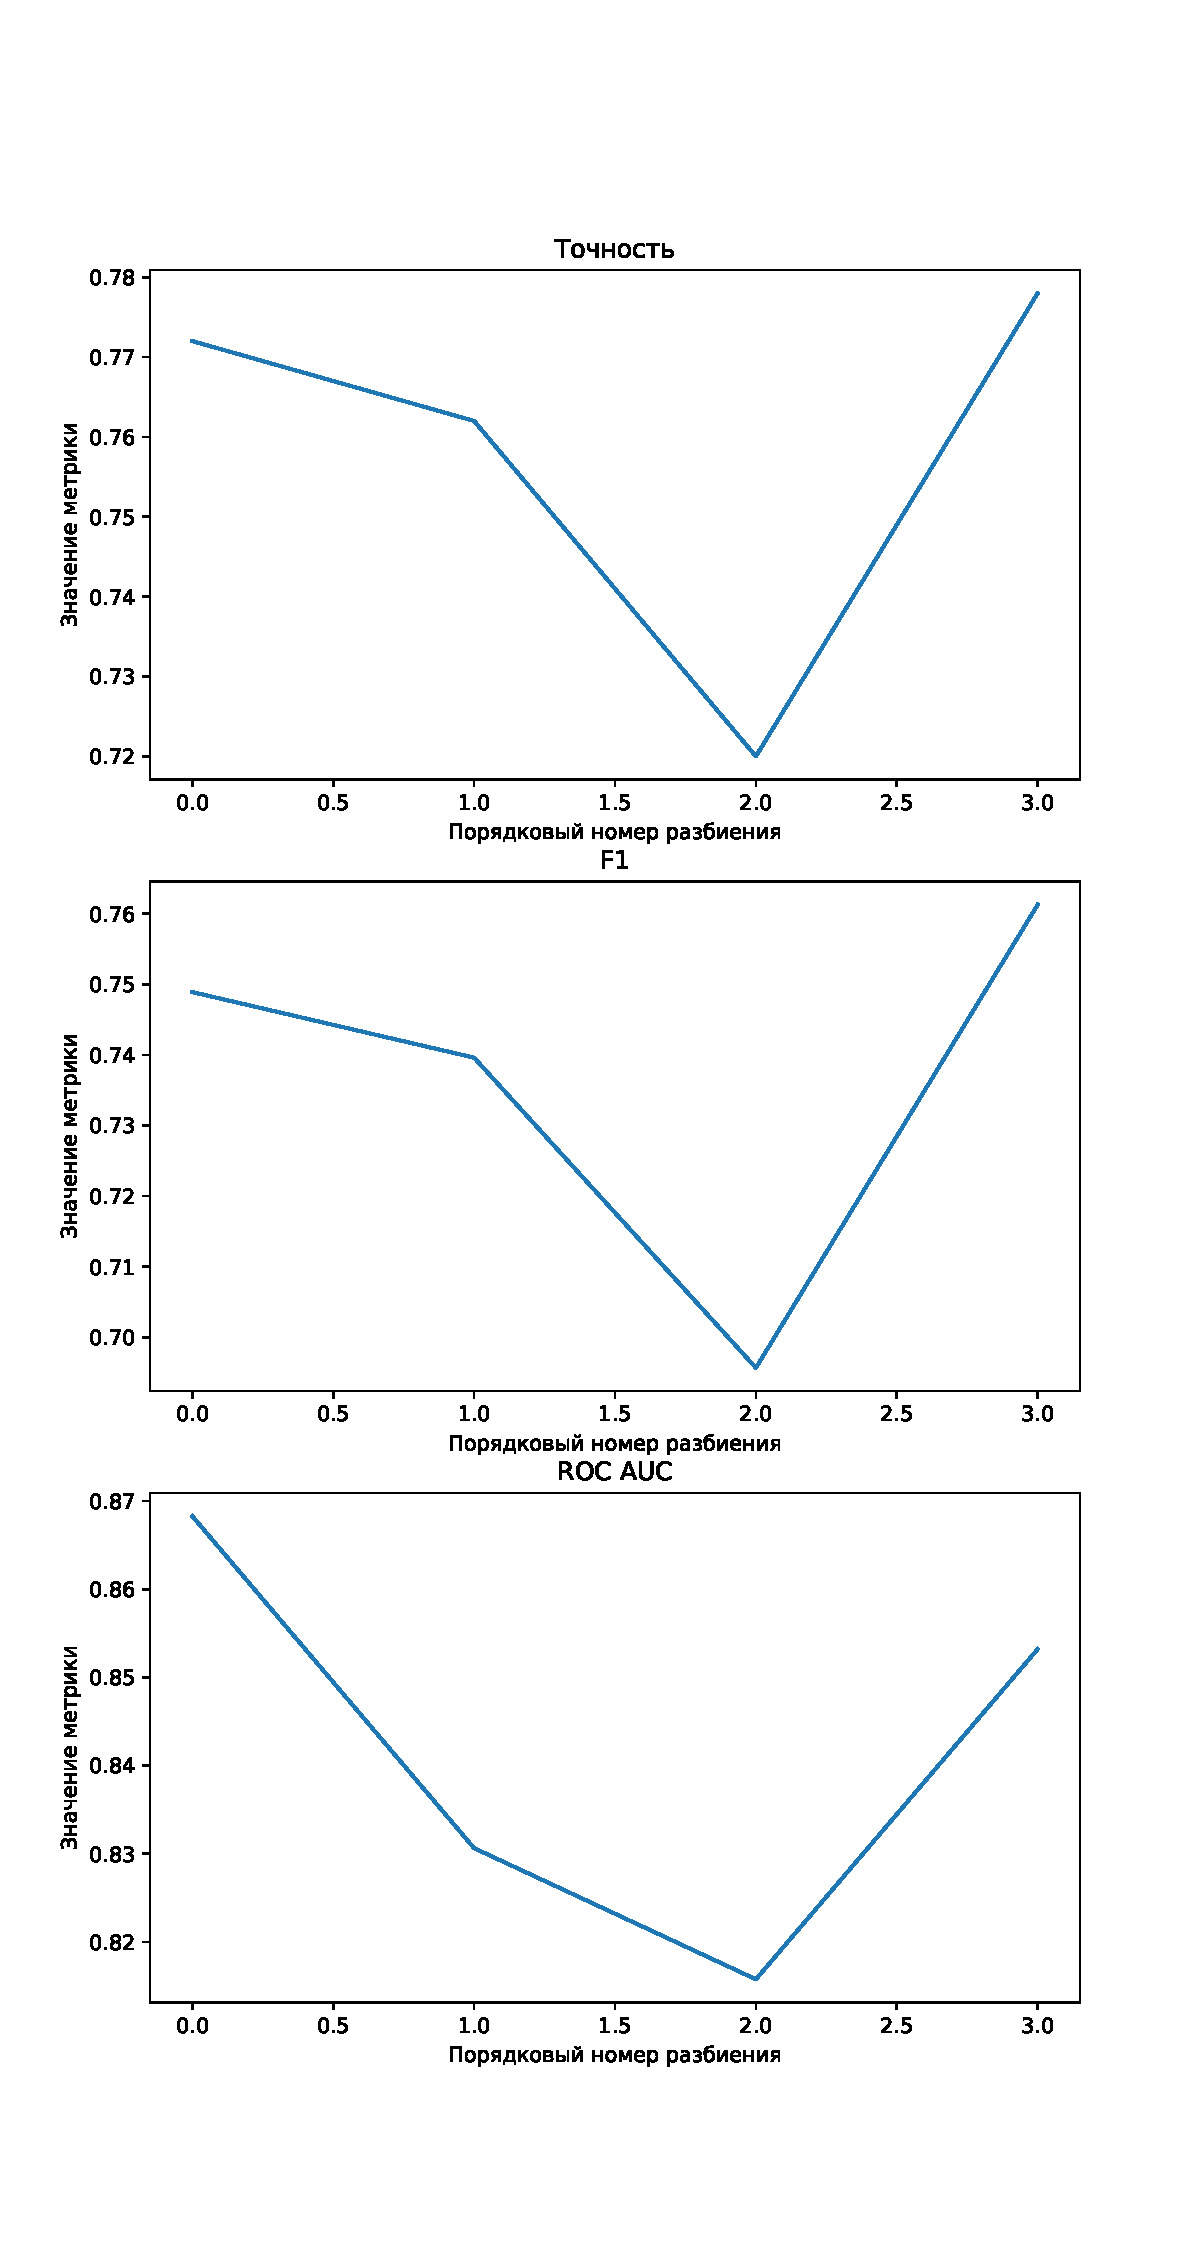
\includegraphics[height=23cm]{inc/plots/knnMetricsBert.pdf}
	\caption{ Оценки классификатора в зависимости от номера разбиения, полученные с использованием метода K-ближайших соседей (метод векторизации -- BERT). }
	\label{img:knnMetricsBert}
\end{figure}



\subsection{Логистическая регрессия }

Параметры модели при применении метода векторизации ``мешок слов'':
\begin{itemize}
	\item регуляризационный параметр -- 2.2;
	\item веса классов -- сбалансированно;
	\item штраф -- определяет тип штрафа, используемого для регуляризации -- сумма квадратов весов модели, умноженных на гиперпараметр регуляризации;
	\item алгоритм оптимизации -- liblinear.
\end{itemize}

На рисунке \ref{img:logicMatrBag} представлены матрицы ошибок, полученные с использованием логистической регрессии, метод векторизации -- ``мешок слов''.
\begin{figure}[H]
	\centering
	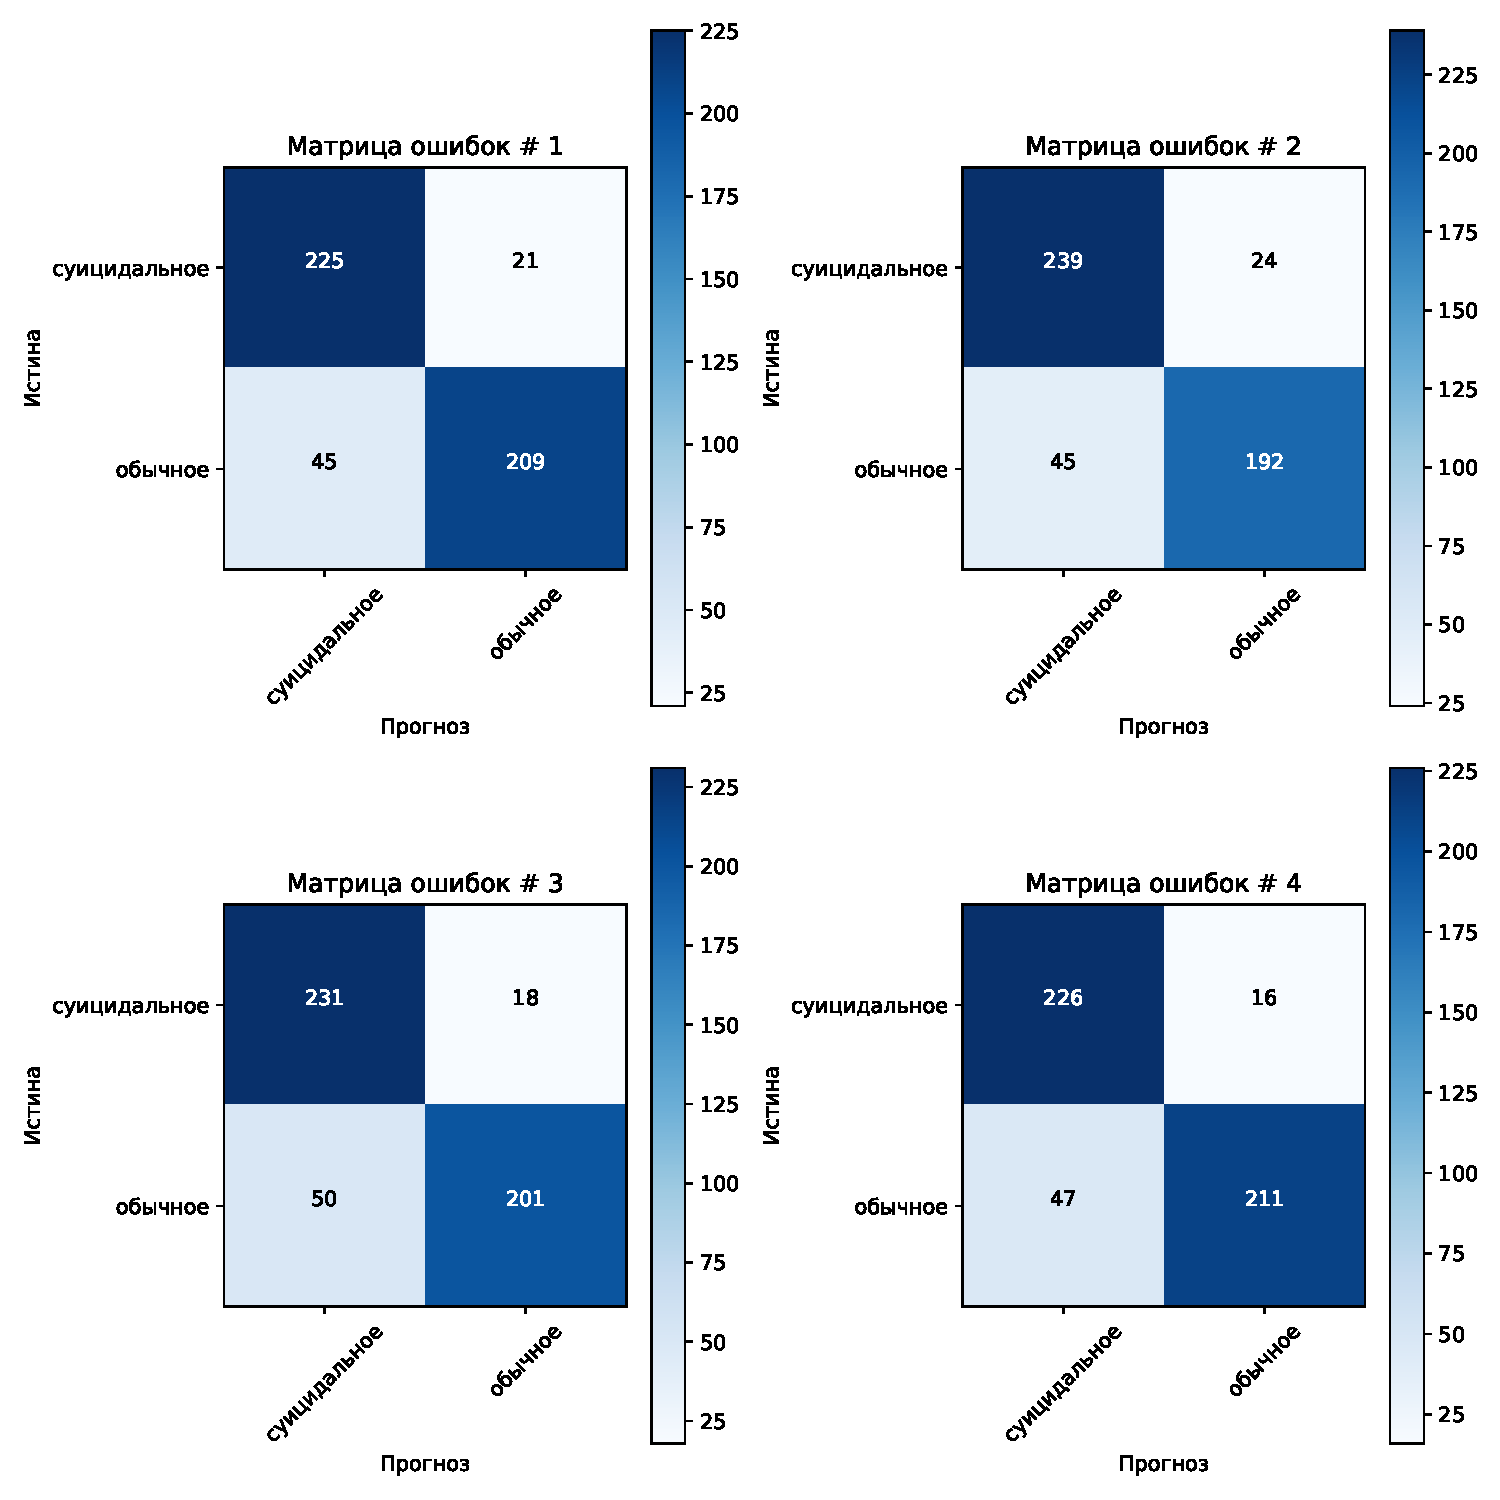
\includegraphics[width=\textwidth]{inc/plots/logicMatrBag.pdf}
	\caption{ Матрицы ошибок в зависимости от номера разбиения, полученные с использованием логистической регрессии (метод векторизации -- ``мешок слов''). }
	\label{img:logicMatrBag}
\end{figure}

На рисунке \ref{img:logicMetricsBag} представлены оценки классификатора, полученные с использованием логистической регрессии, метод векторизации -- ``мешок слов''.
\begin{figure}[H]
	\centering
	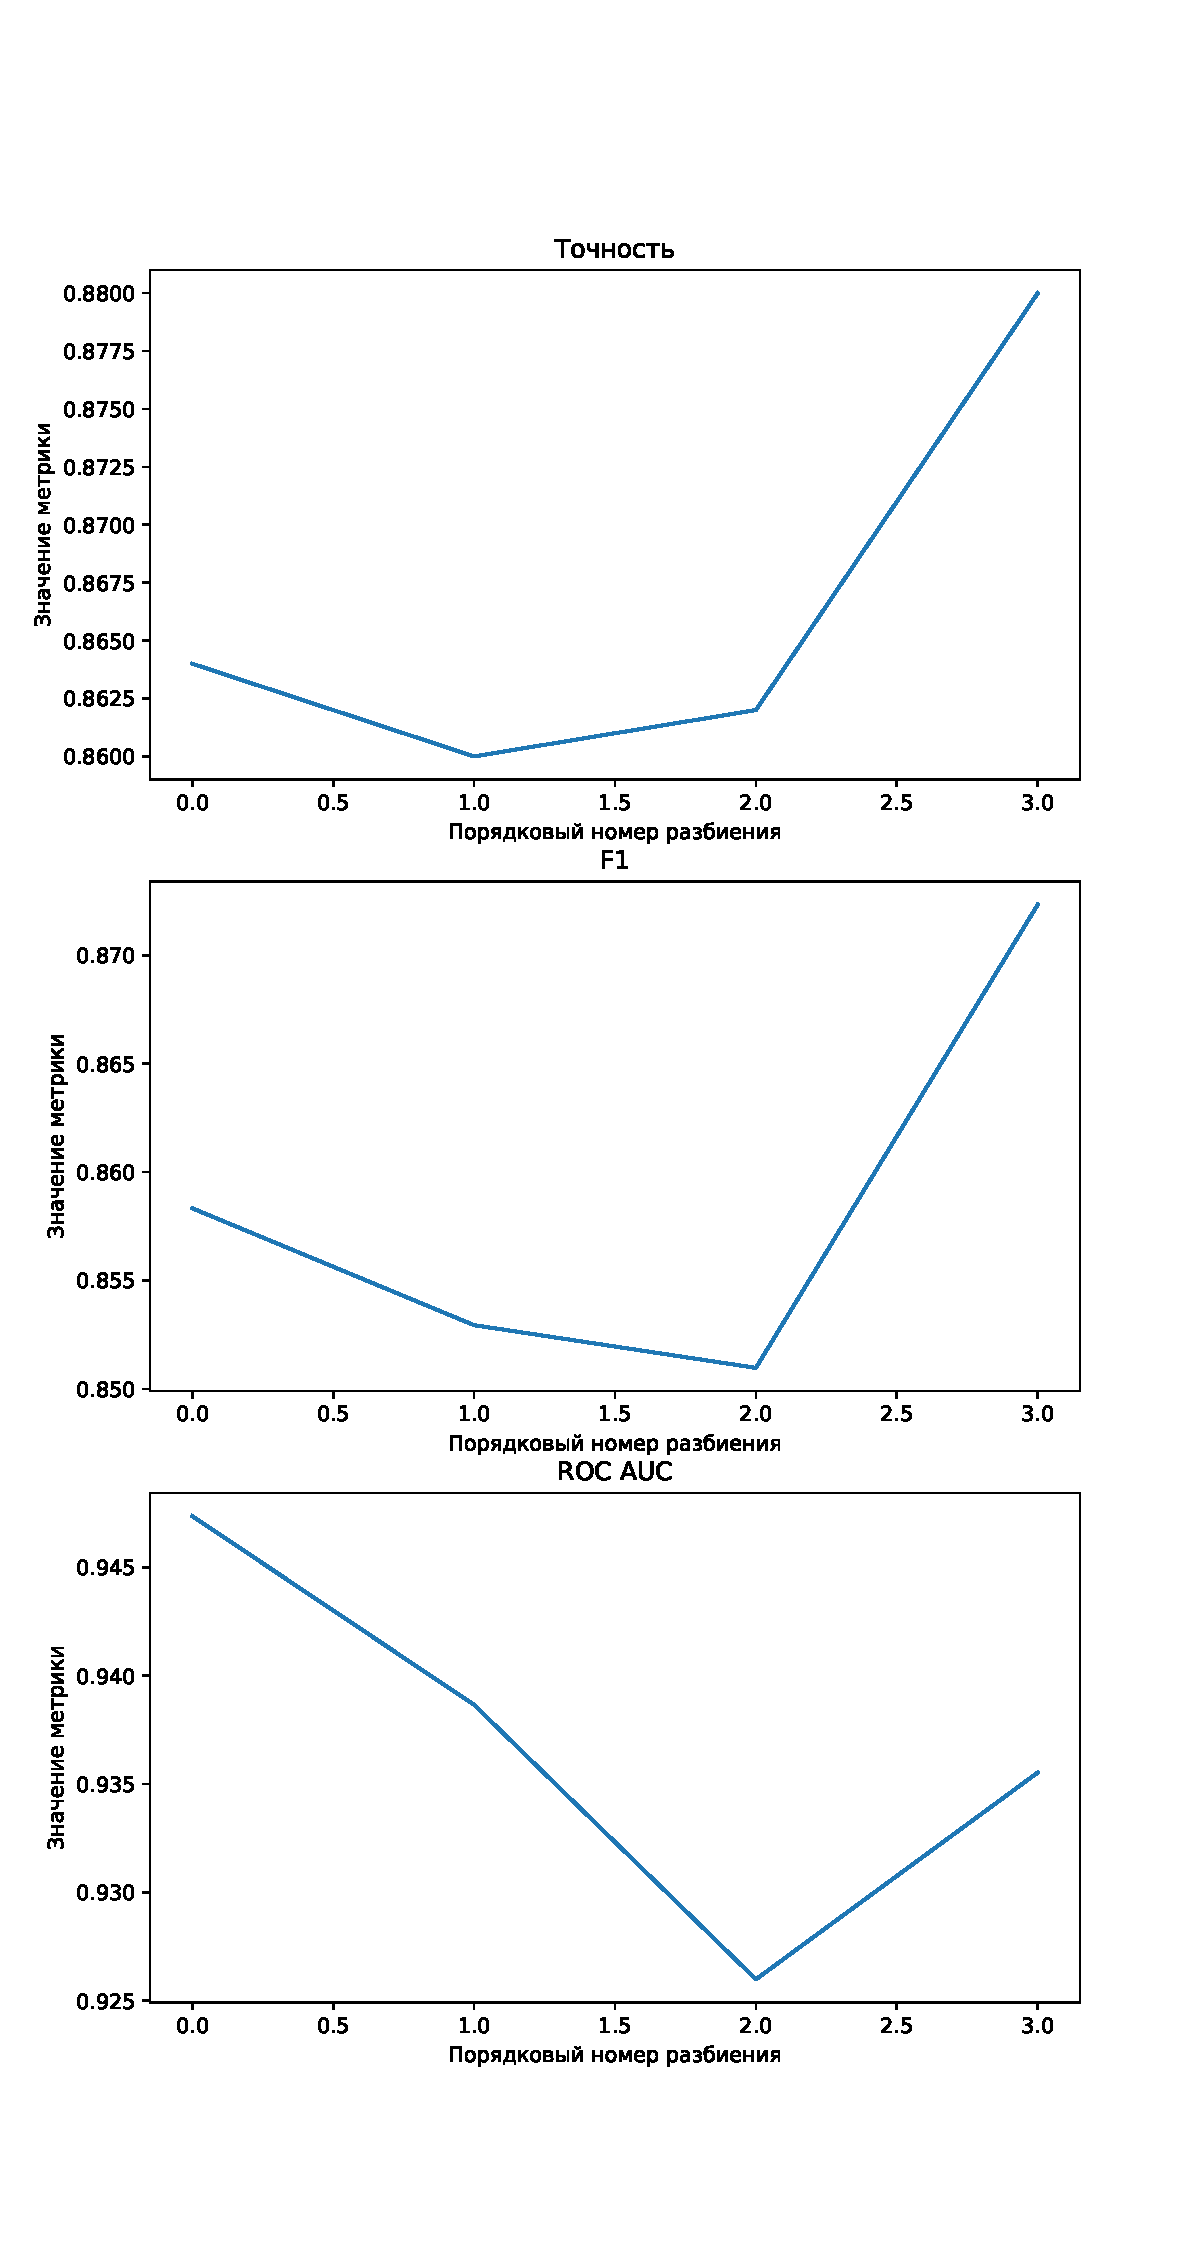
\includegraphics[height=23cm]{inc/plots/logicMetricsBag.pdf}
	\caption{ Оценки классификатора в зависимости от номера разбиения, полученные с использованием логистической регрессии (метод векторизации --  ``мешок слов''). }
	\label{img:logicMetricsBag}
\end{figure}


Параметры модели при применении векторизации BERT:
\begin{itemize}
	\item регуляризационный параметр -- 2.1;
	\item веса классов -- сбалансированно;
	\item штраф -- сумма квадратов весов модели, умноженных на гиперпараметр регуляризации;
	\item алгоритм оптимизации -- liblinear.
\end{itemize}
На рисунке \ref{img:logicMatrBert} представлены матрицы ошибок, полученные с использованием логистической регрессии, метод векторизации -- BERT.

\begin{figure}[H]
	\centering
	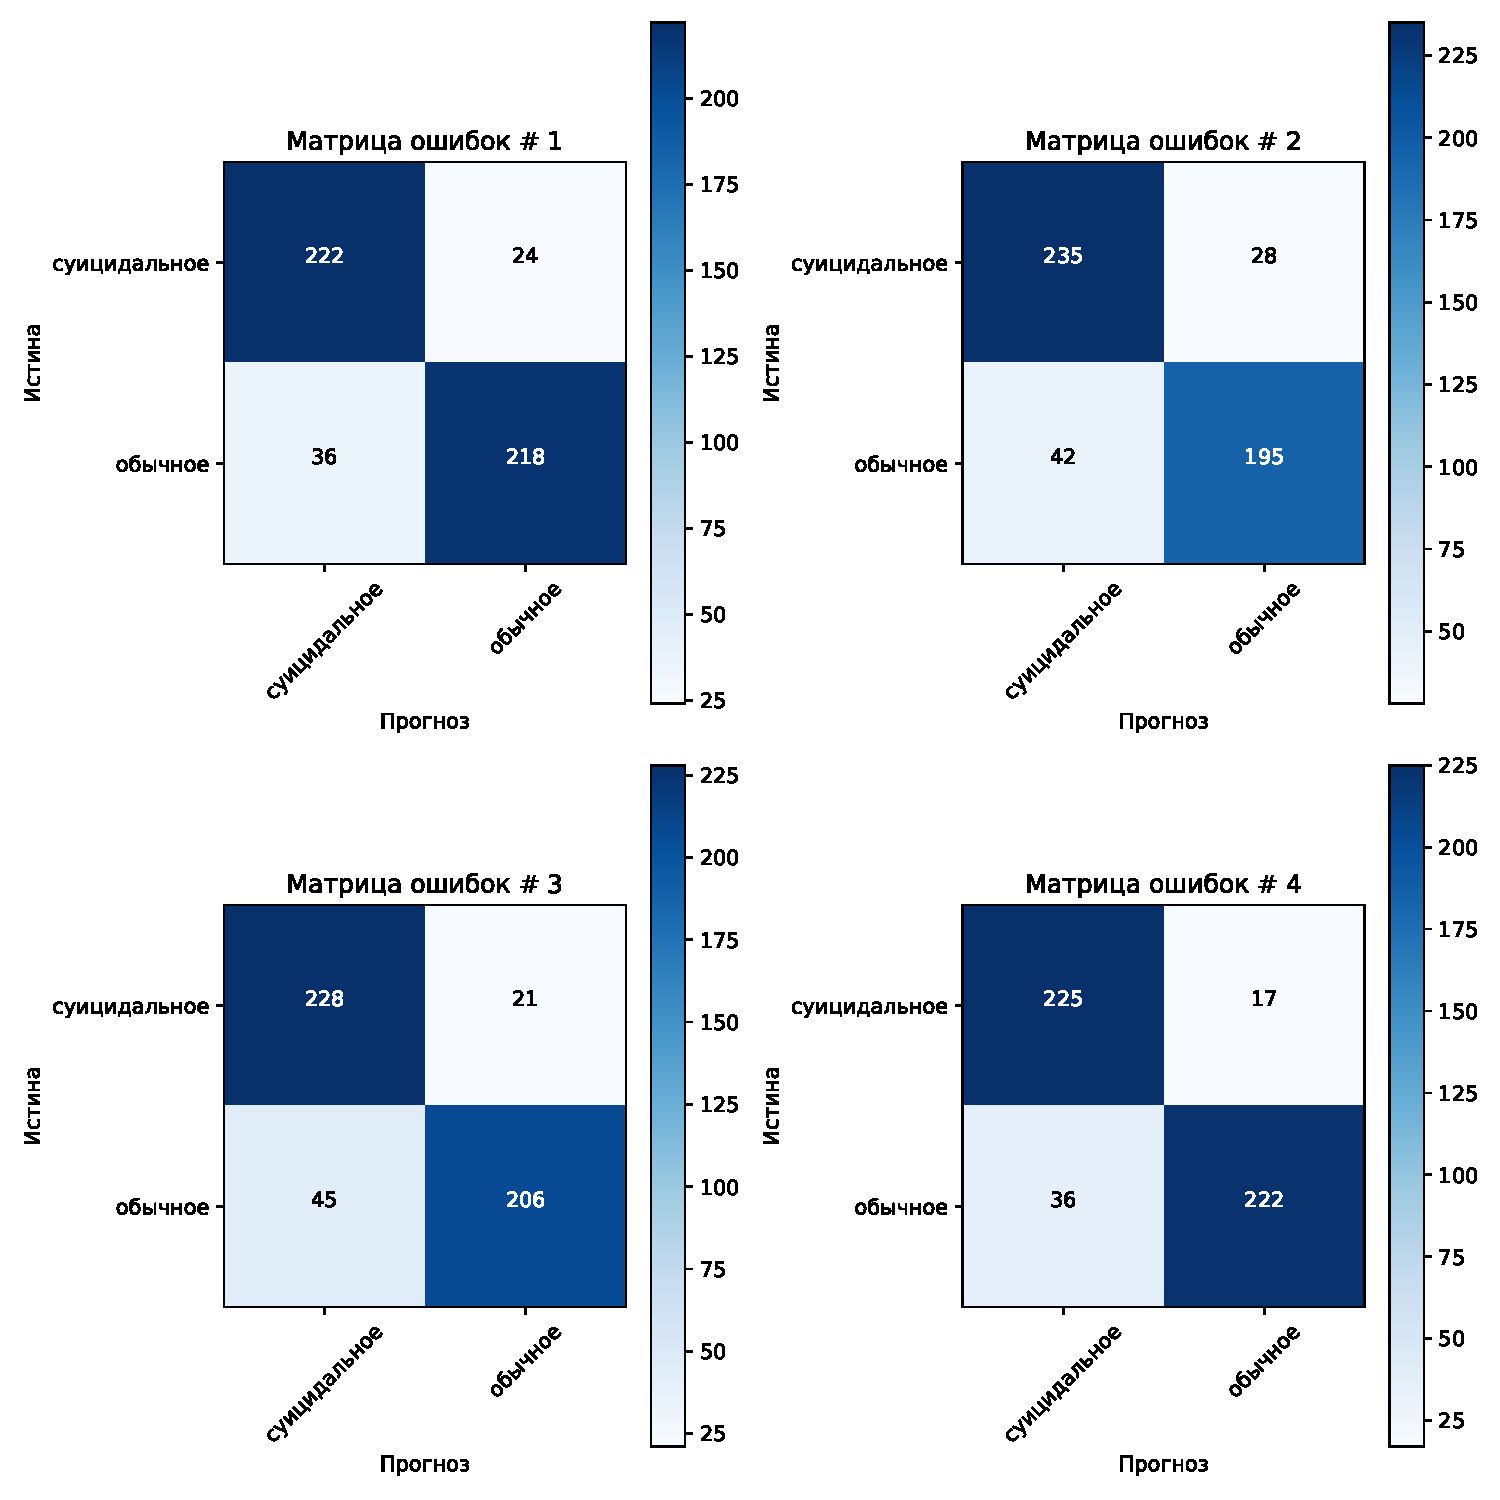
\includegraphics[width=\textwidth]{inc/plots/logicMatrBert.pdf}
	\caption{ Матрицы ошибок в зависимости от номера разбиения, полученные с использованием логистической регрессии (метод векторизации -- BERT). }
	\label{img:logicMatrBert}
\end{figure}

На рисунке \ref{img:logicMetricsBert} представлены оценки классификатора, полученные с использованием логистической регрессии, метод векторизации -- BERT.
\begin{figure}[H]
	\centering
	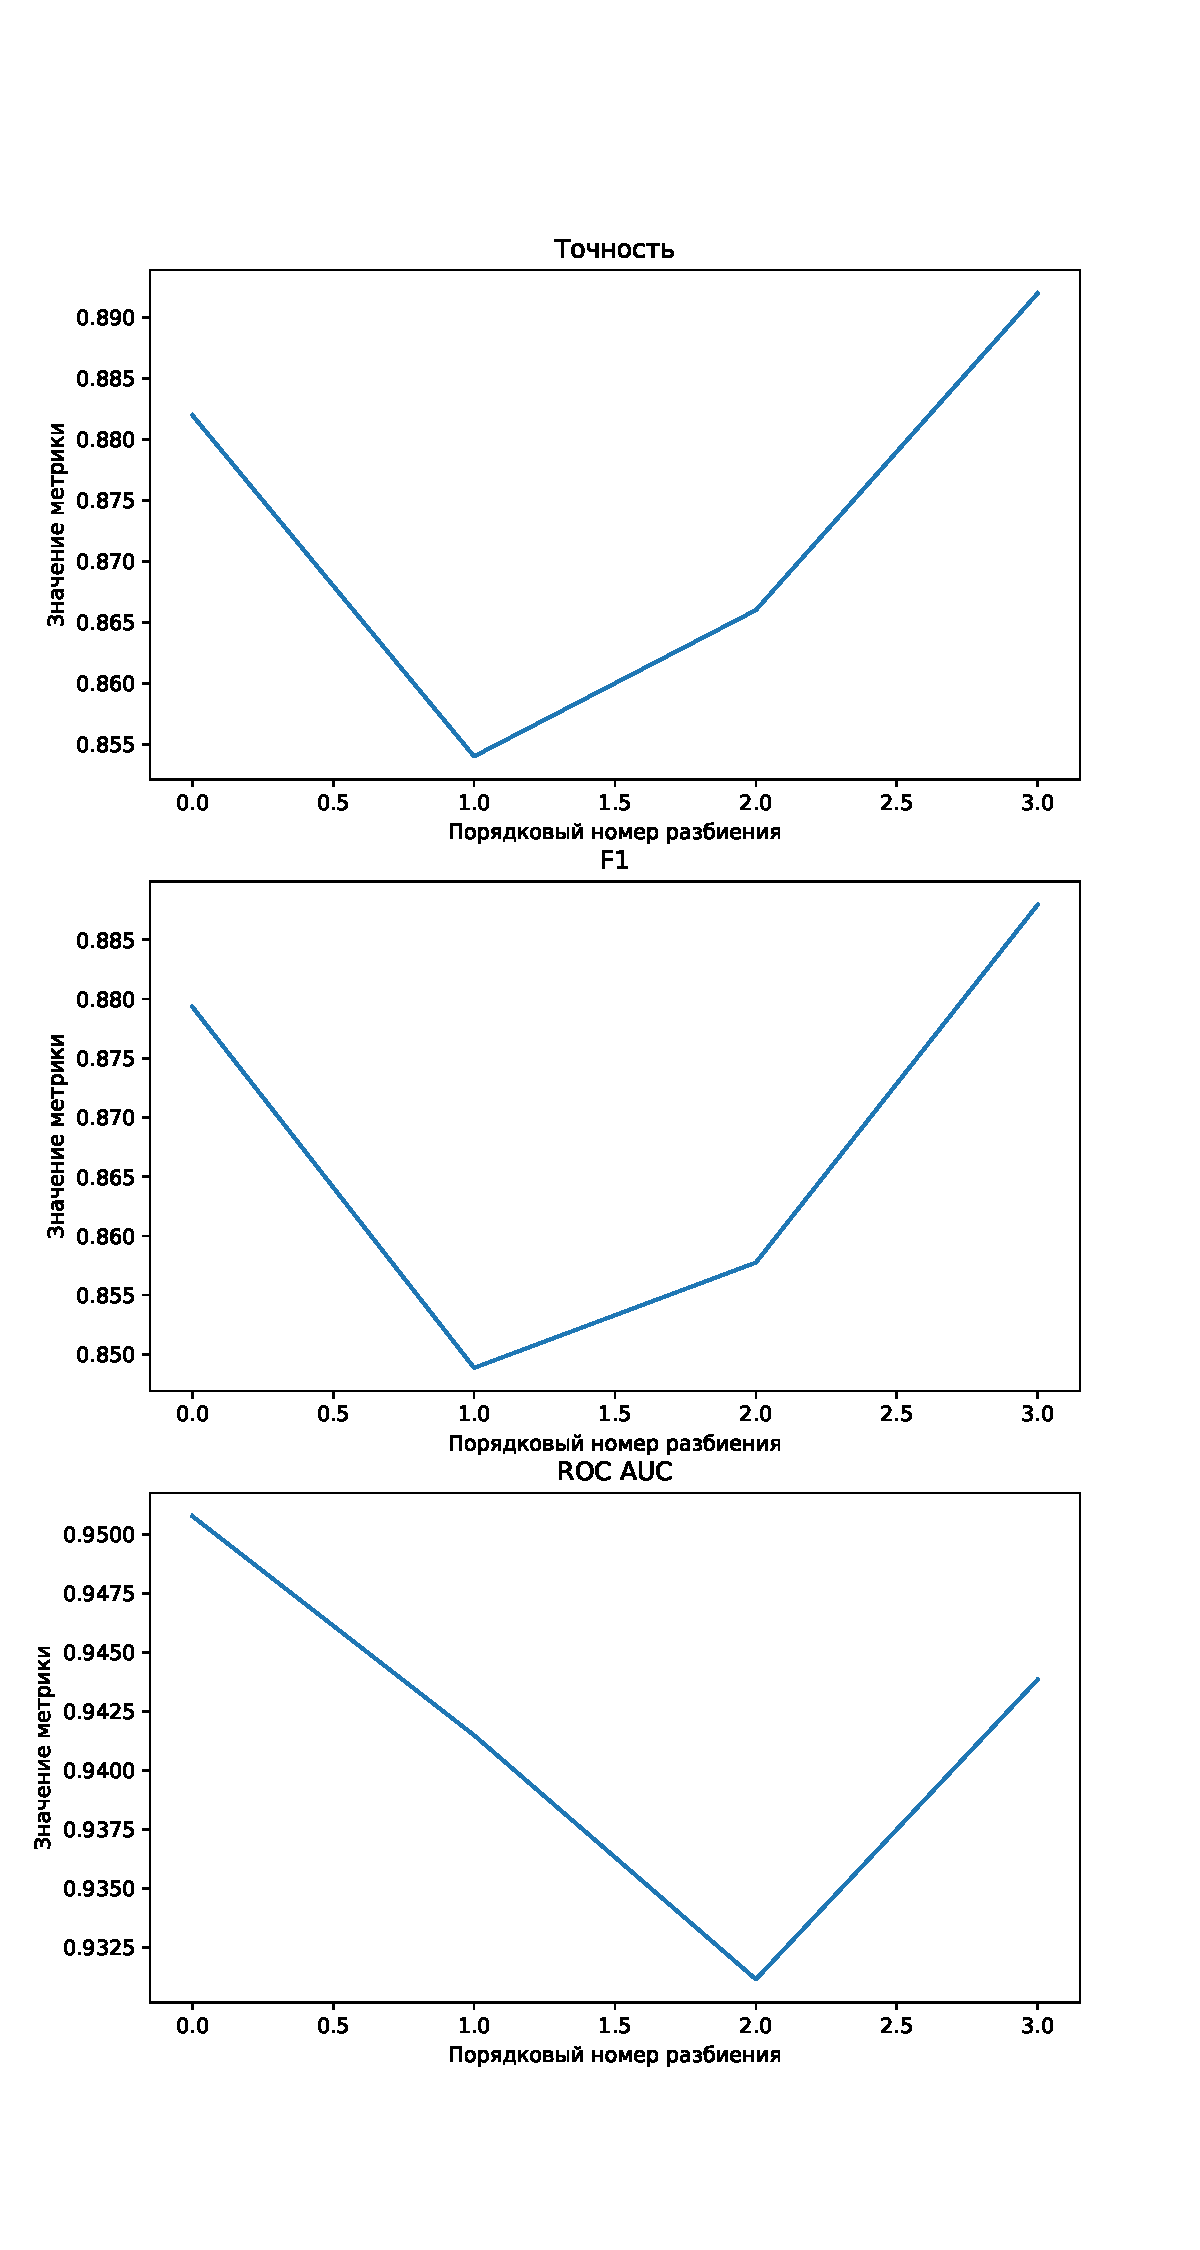
\includegraphics[height=23cm]{inc/plots/logicMetricsBert.pdf}
	\caption{ Оценки классификатора в зависимости от номера разбиения, полученные с использованием логистической регрессии (метод векторизации -- BERT). }
	\label{img:logicMetricsBert}
\end{figure}



\subsection{Перцептрон }

Параметры модели при применении метода векторизации ``мешок слов'':
\begin{itemize}
	\item скорость обучения -- 0.0001;
	\item максимальное количество итераций при обучении -- 30;
	\item штраф -- сумма квадратов весов модели, умноженных на гиперпараметр регуляризации.
\end{itemize}

На рисунке \ref{img:perceptronMatrBag} представлены матрицы ошибок, полученные с использованием перцептрона, метод векторизации -- ``мешок слов''.
\begin{figure}[H]
	\centering
	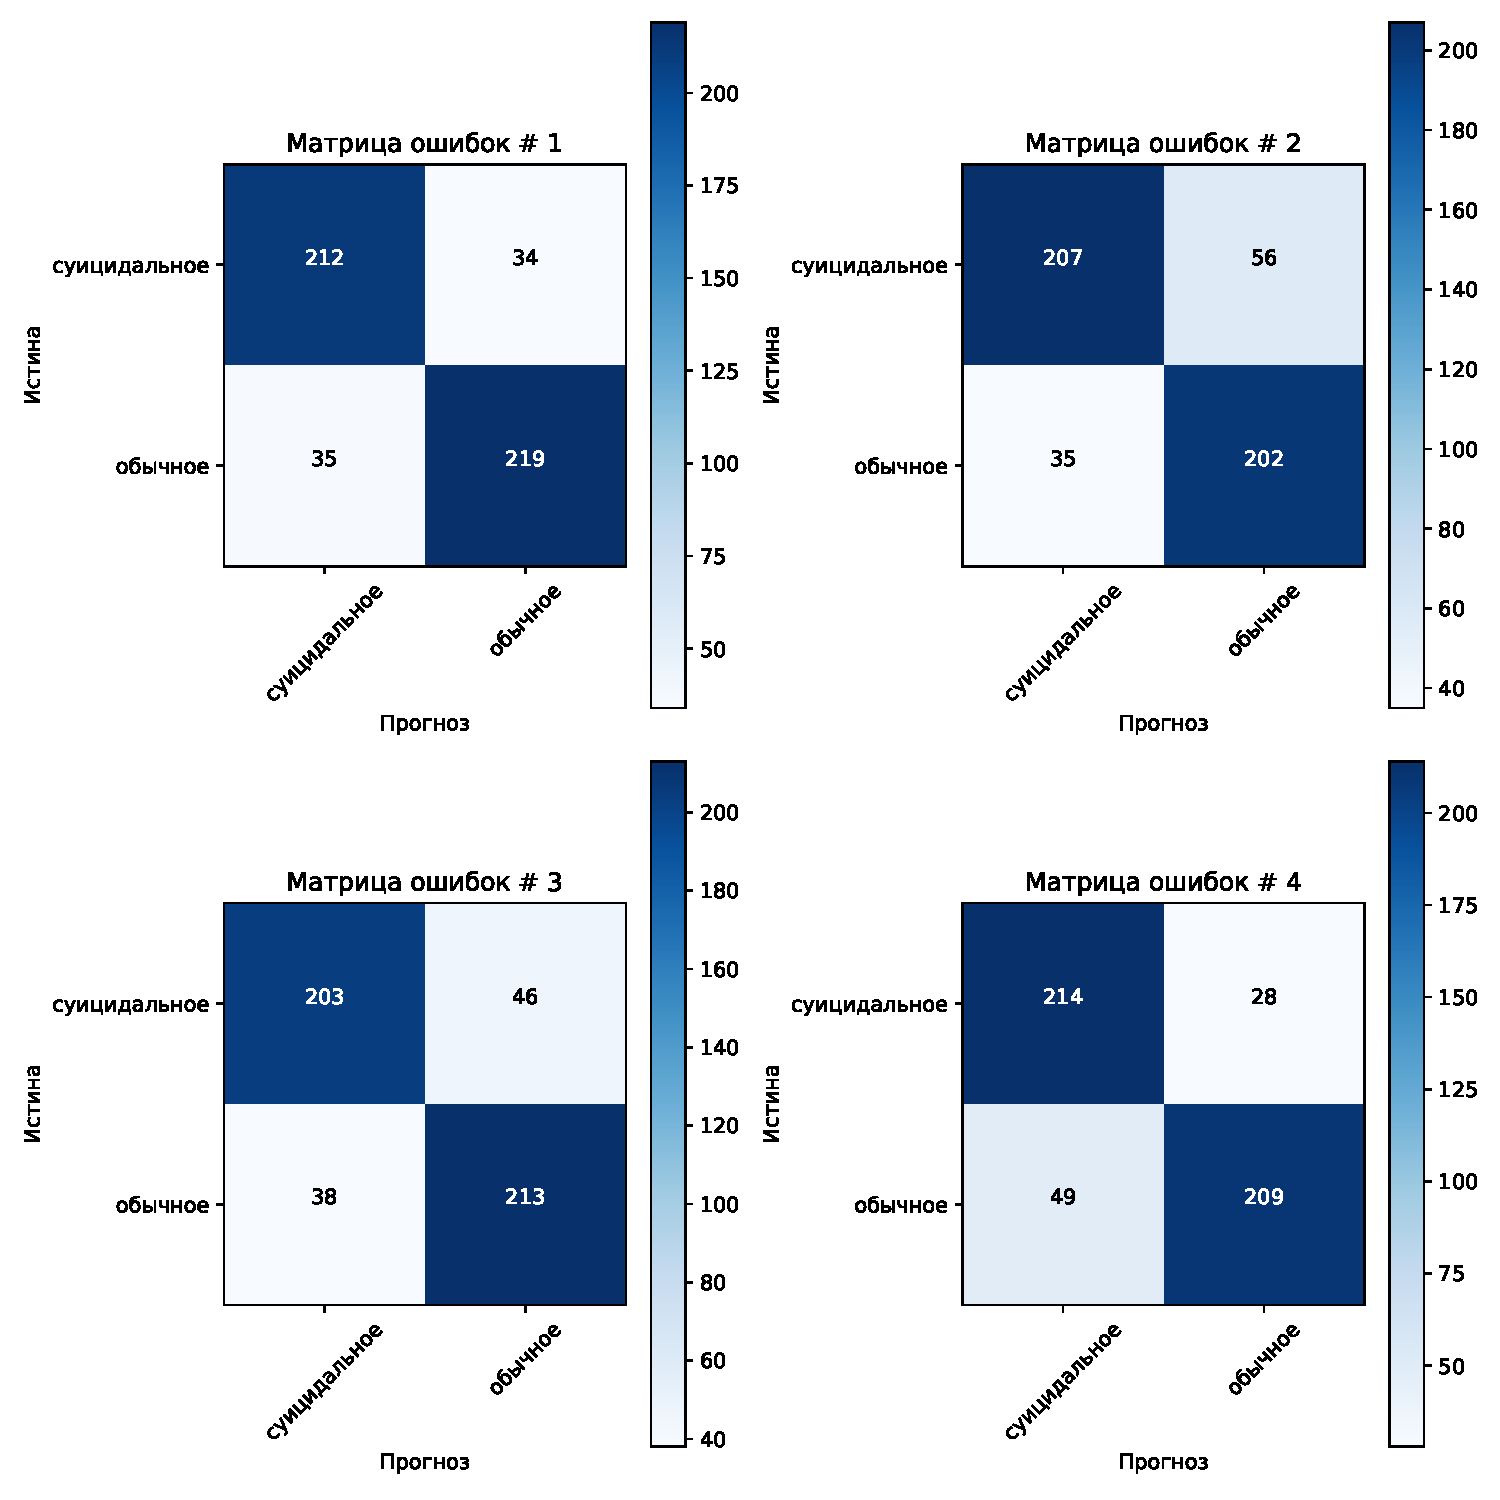
\includegraphics[width=\textwidth]{inc/plots/perceptronMatrBag.pdf}
	\caption{ Матрицы ошибок в зависимости от номера разбиения, полученные с использованием перцептрона (метод векторизации -- ``мешок слов''). }
	\label{img:perceptronMatrBag}
\end{figure}

На рисунке \ref{img:perceptronMetricsBag} представлены оценки классификатора, полученные с использованием перцептрона, метод векторизации -- ``мешок слов''.
\begin{figure}[H]
	\centering
	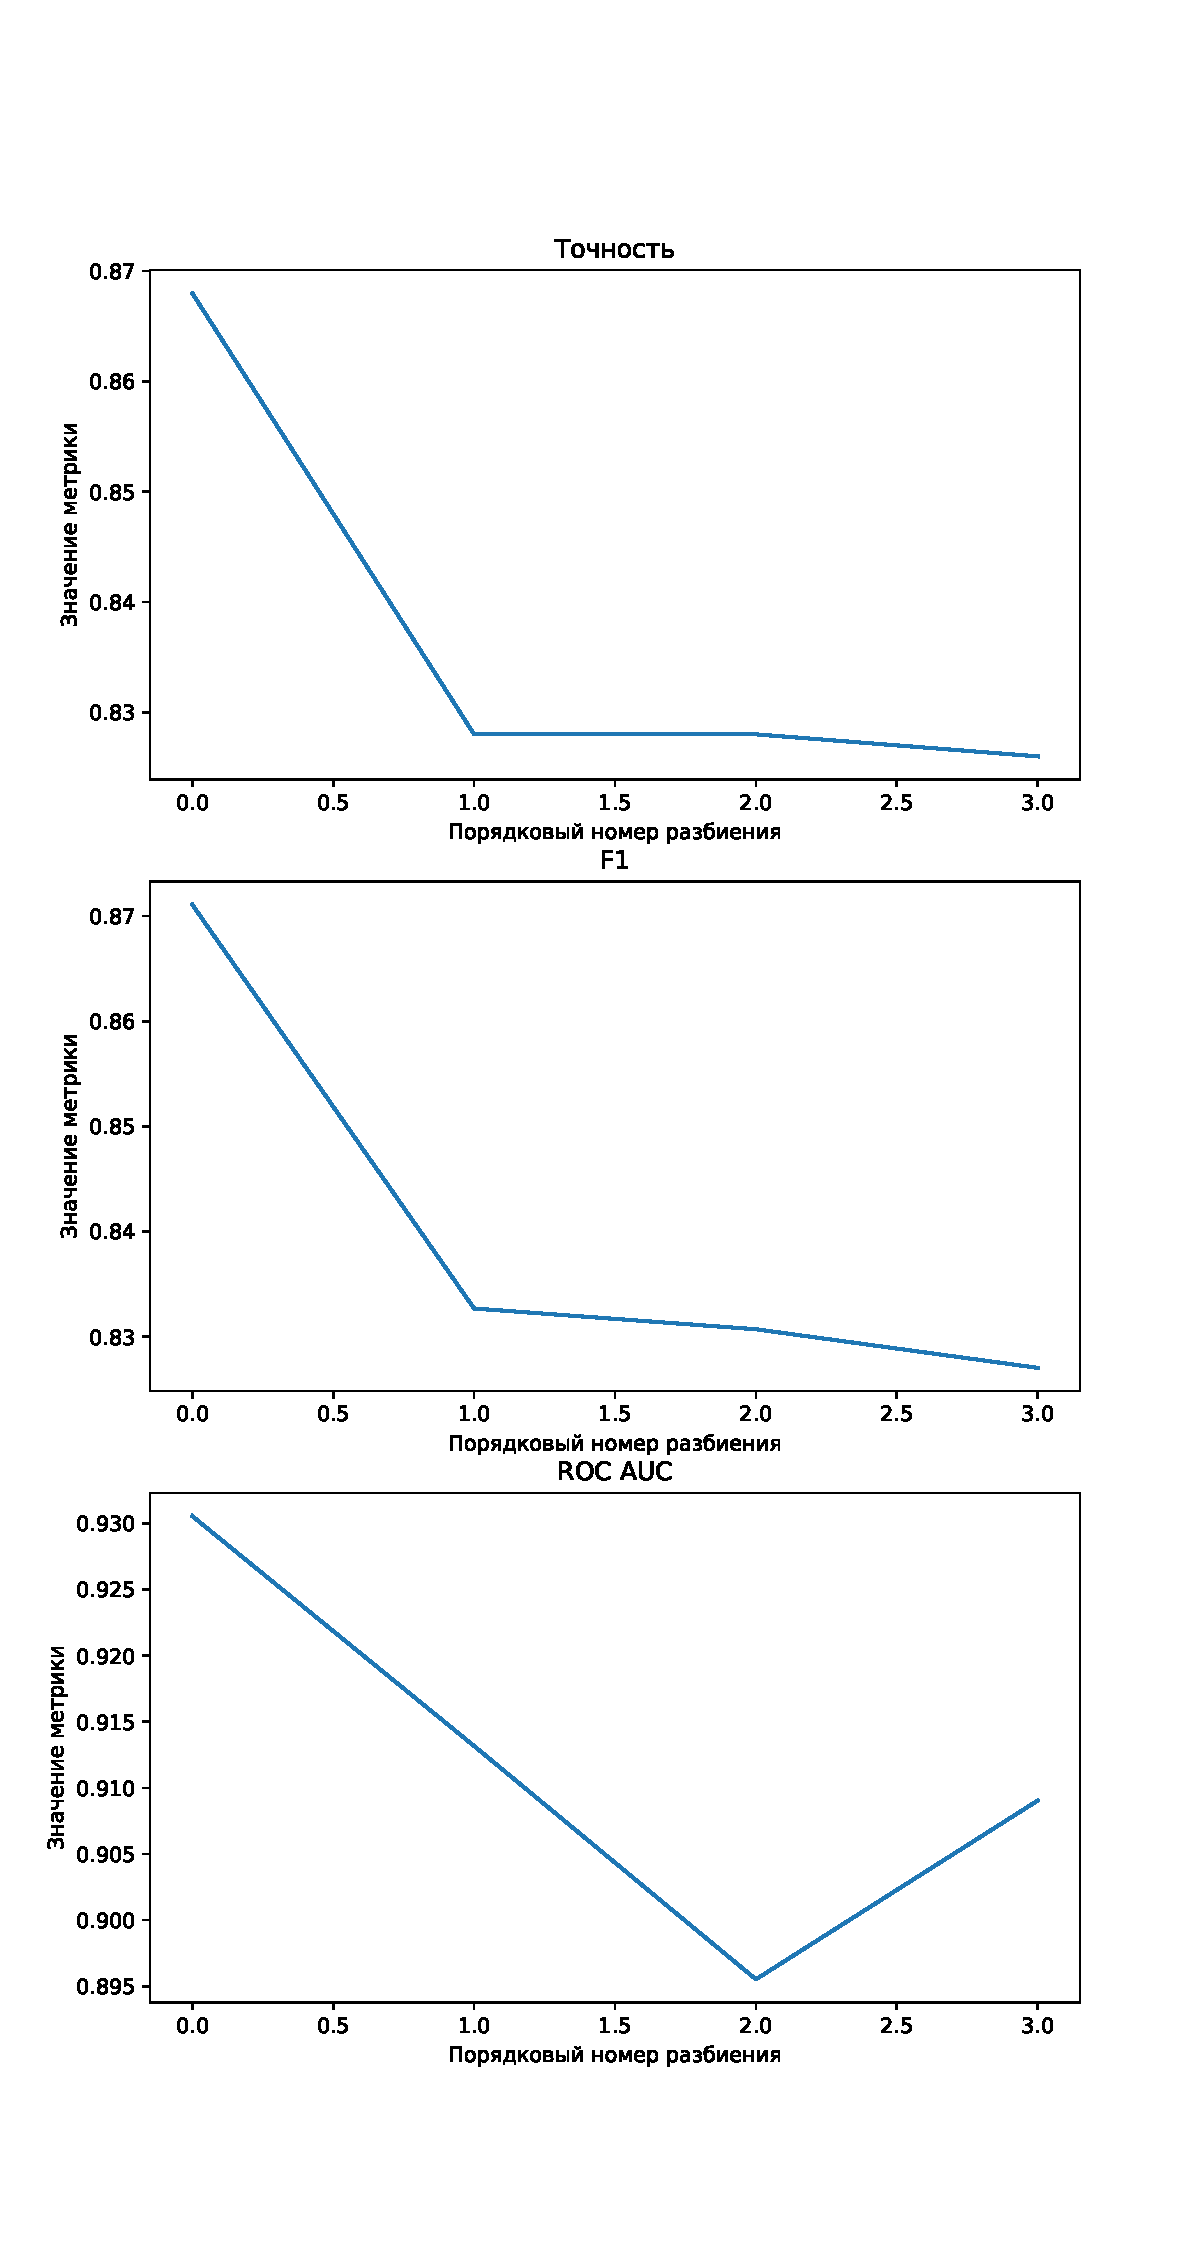
\includegraphics[height=23cm]{inc/plots/perceptronMetricsBag.pdf}
	\caption{ Оценки классификатора в зависимости от номера разбиения, полученные с использованием перцептрона (метод векторизации --  ``мешок слов''). }
	\label{img:perceptronMetricsBag}
\end{figure}


Параметры модели при применении векторизации BERT:
\begin{itemize}
	\item скорость обучения -- 0.0001;
	\item максимальное количество итераций при обучении -- 30;
	\item штраф -- абсолютное значение коэффициентов модели.
\end{itemize}

На рисунке \ref{img:perceptronMatrBert} представлены матрицы ошибок, полученные с использованием перцептрона, метод векторизации -- BERT.
\begin{figure}[H]
	\centering
	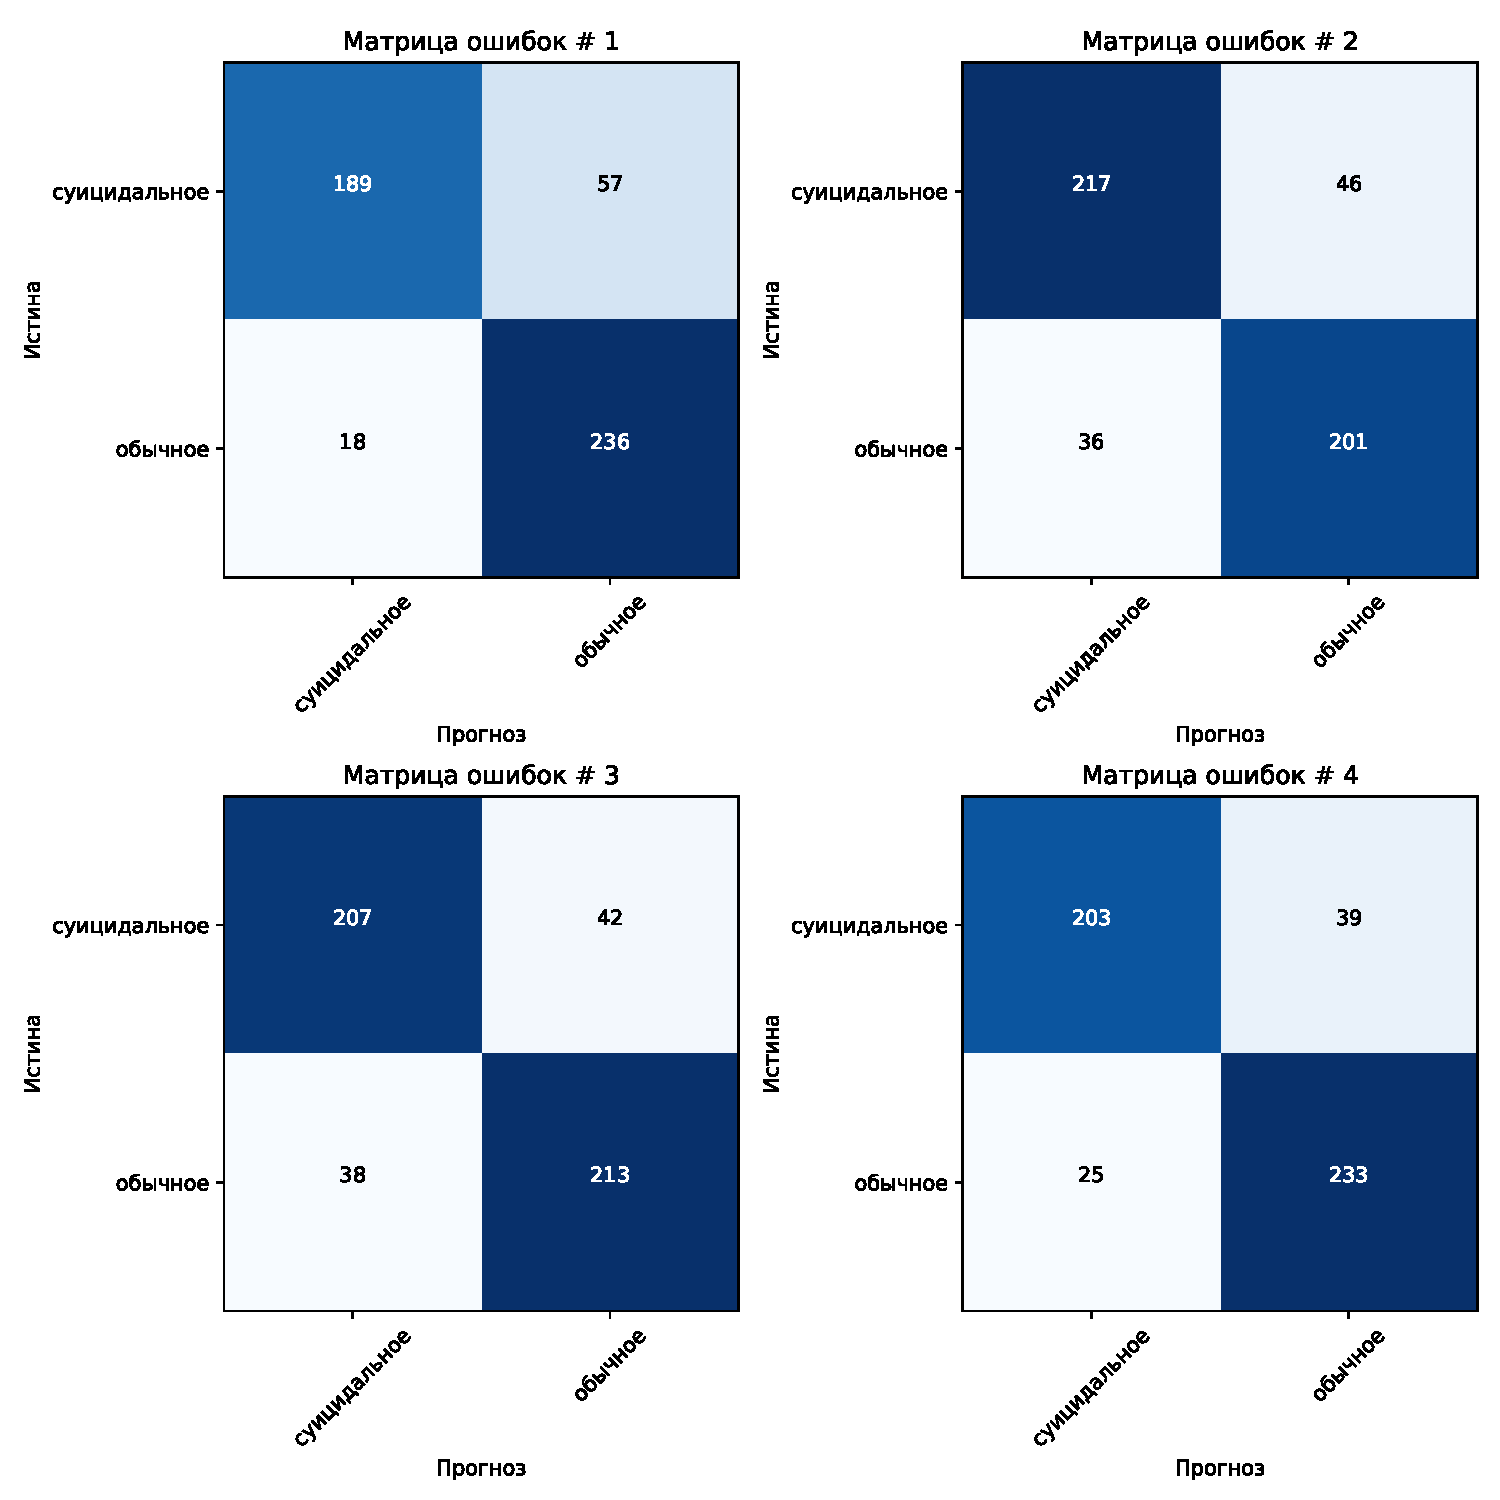
\includegraphics[width=\textwidth]{inc/plots/perceptronMatrBert.pdf}
	\caption{ Матрицы ошибок в зависимости от номера разбиения, полученные с использованием перцептрона (метод векторизации -- BERT). }
	\label{img:perceptronMatrBert}
\end{figure}

На рисунке \ref{img:perceptronMetricsBert} представлены оценки классификатора, полученные с использованием перцептрона, метод векторизации -- BERT.
\begin{figure}[H]
	\centering
	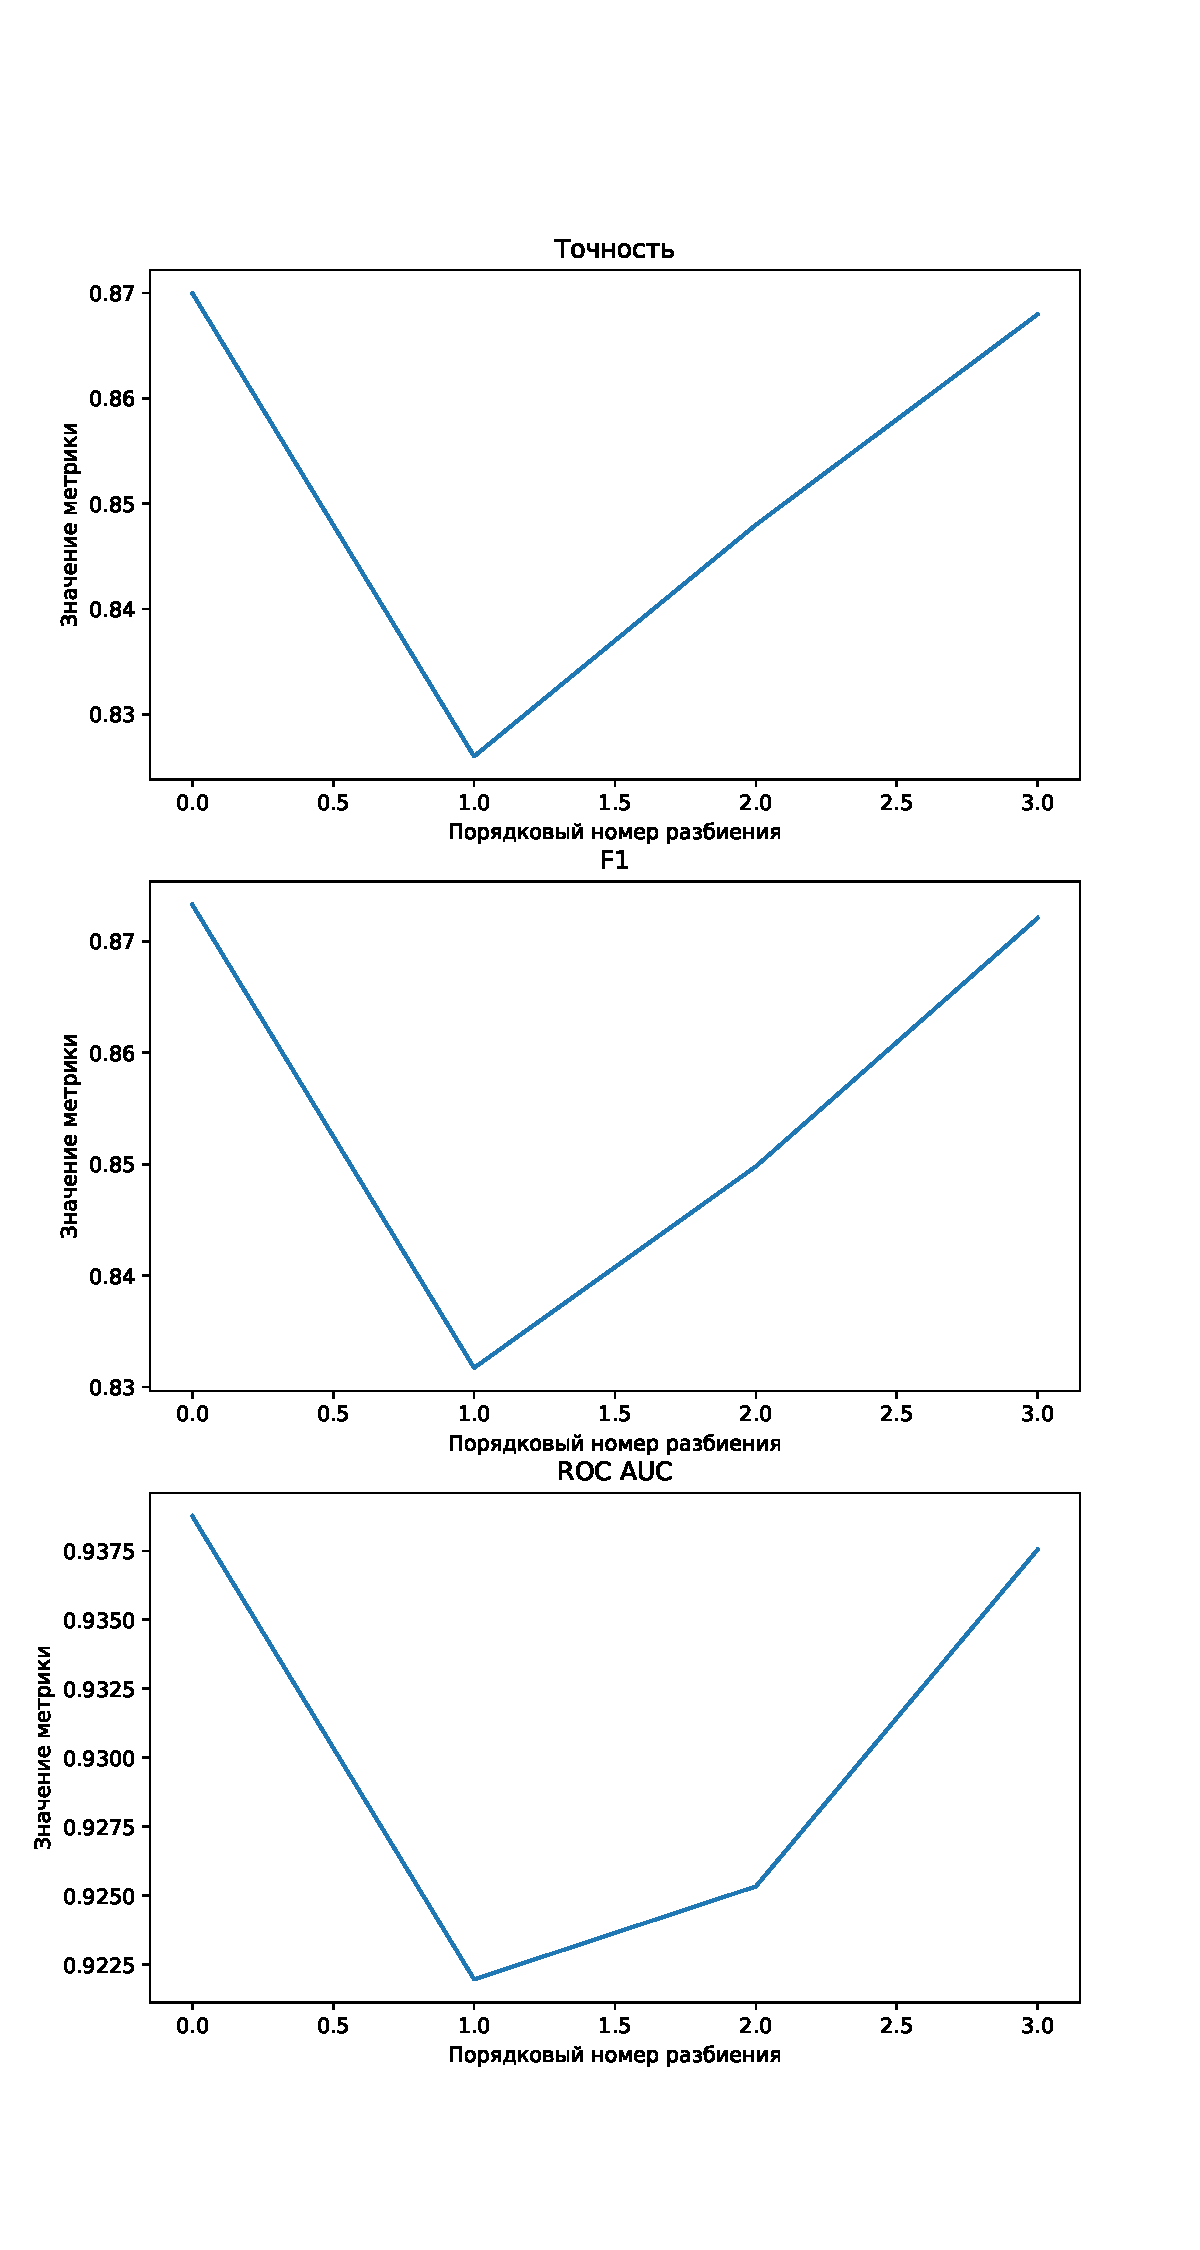
\includegraphics[height=23cm]{inc/plots/perceptronMetricsBert.pdf}
	\caption{ Оценки классификатора в зависимости от номера разбиения, полученные с использованием перцептрона (метод векторизации -- BERT). }
	\label{img:perceptronMetricsBert}
\end{figure}

\subsection{Интерпретация результатов}

По представленным матрицам ошибок можно увидеть, что все методы, кроме случайного леса (BERT), метода опорных векторов (оба варианта векторизации) и перцептрона (оба варианта), в большинстве своем в 2 раза чаще определяют обычное сообщение как суицидальное. Метод опорных векторов имеет более распределенные матрицы ошибок. Самые частые ошибки в определении обычных сообщений совершал метод К-ближайших соседей. Перцептрон на каждом из разбиений мог либо хуже распознавать суицидальные, либо хуже распознавать обычные сообщения.

В таблицах \ref{table:result1} и \ref{table:result2} представлены результаты проведенного исследования, в которых для каждого алгоритма выделены лучшие показатели каждой метрики.

\begin{table}[H]
	\begin{center}
		\captionsetup{justification=centering}
		\caption{\label{table:result1} Результаты исследования}
		\begin{tabular}{|p{3cm}|p{4cm}|p{2.5cm}|p{2.5cm}|p{2.5cm}|}
				\hline
			Алгоритм & Векторизация & Точность & F1-мера & ROC-AUC \\
				\hline\hline
			
			\multirow{10}{*}{\shortstack[l]{Градиентный \\ бустинг}} 
			& ``Мешок слов'' & 0.854 & 0.852 & 0.928 \\
				& & 0.840 & 0.830 & 0.910 \\
				& & 0.860 & 0.835 & 0.910 \\
				& & 0.858 & 0.853 & 0.927 \\
				\cline{2-5} & \textit{среднее} & \textit{0.853} & \textit{0.843} & \textit{0.919} \\
			\cline{2-5}
			& BERT & 0.852 & 0.848 & 0.936 \\
				& & 0.848 & 0.831 & 0.916 \\
				& & 0.856 & 0.849 & 0.926 \\
				& & 0.890 & 0.878 & 0.939 \\
				\cline{2-5} & \textit{среднее} & \textit{0.862} & \textit{0.852} & \textit{0.929} \\
			\hline\hline
			
			\multirow{8}{*}{\shortstack[l]{Случайный \\ лес}} 
			& ``Мешок слов'' & 0.876 & 0.875 & 0.952 \\
				&& 0.862 & 0.868 & 0.940 \\
				&& 0.890 & 0.879 & 0.938 \\
				&& 0.882 & 0.879 & 0.957 \\
				\cline{2-5} & \textit{среднее} & \textit{0.878} & \textit{0.875} & \textit{0.947} \\
			\cline{2-5}
			& BERT & 0.888 & 0.886 & 0.952 \\
				&& 0.890 & 0.887 & 0.945 \\
				&& 0.880 & 0.873 & 0.935 \\
				&& 0.892 & 0.900 & 0.960 \\
				\cline{2-5} & \textit{среднее} & \textbf{\textit{0.888}} & \textbf{\textit{0.887}} & \textbf{\textit{0.948}} \\
			\hline\hline
			
			\multirow{8}{*}{\shortstack[l]{Метод\\опорных\\векторов}} 
			& ``Мешок слов'' & 0.850 & 0.851 & 0.924 \\
				& & 0.848 & 0.847 & 0.920 \\
				& & 0.824 & 0.819 & 0.899 \\
				& & 0.864 & 0.862 & 0.918 \\
				\cline{2-5} & \textit{среднее} & \textit{0.847} & \textit{0.845} & \textit{0.915} \\
			\cline{2-5}
			& BERT & 0.864 & 0.865 & 0.930 \\
				& & 0.850 & 0.850 & 0.921 \\
				& & 0.848 & 0.844 & 0.919 \\
				& & 0.886 & 0.884 & 0.928 \\
				\cline{2-5} & \textit{среднее} & \textit{0.862} & \textit{0.861} & \textit{0.925} \\
					
			\hline
		\end{tabular}
	\end{center}
\end{table}

\begin{table}[H]
	\begin{center}
		\captionsetup{justification=centering}
		\caption{\label{table:result2} Результаты исследования}
		\begin{tabular}{|p{3cm}|p{4cm}|p{2.5cm}|p{2.5cm}|p{2.5cm}|}
				\hline
			Алгоритм & Векторизация & Точность & F1-мера & ROC-AUC \\
				\hline\hline
				
			\multirow{8}{*}{\shortstack[l]{Метод\\К-ближайших\\соседей}} 
			& ``Мешок слов'' & 0.742 & 0.692 & 0.854 \\
				& & 0.750 & 0.691 & 0.844 \\
				& & 0.738 & 0.678 & 0.845 \\
				& & 0.778 & 0.754 & 0.874 \\
				\cline{2-5} & \textit{среднее} & \textit{0.752} & \textit{0.704} & \textit{0.854} \\
			\cline{2-5}
			& BERT & 0.772 & 0.749 & 0.868 \\
				& & 0.762 & 0.740 & 0.831 \\
				& & 0.720 & 0.696 & 0.816 \\
				& & 0.778 & 0.761 & 0.853 \\
				\cline{2-5} & \textit{среднее} & \textit{0.758} & \textit{0.737} & \textit{0.842} \\
			\hline\hline
			
			\multirow{8}{*}{\shortstack[l]{Логистическая\\регрессия}} 
			& ``Мешок слов'' & 0.864 & 0.858 & 0.947 \\
				& & 0.860 & 0.853 & 0.939 \\
				& & 0.862 & 0.851 & 0.926 \\
				& & 0.880 & 0.872 & 0.936 \\
				\cline{2-5} & \textit{среднее} & \textit{0.867} & \textit{0.859} & \textit{0.937} \\
			\cline{2-5}
			& BERT & 0.882 & 0.879 & 0.951 \\
				& & 0.854 & 0.849 & 0.941 \\
				& & 0.866 & 0.858 & 0.931 \\
				& & 0.892 & 0.888 & 0.944 \\
				\cline{2-5} & \textit{среднее} & \textit{0.874} & \textit{0.869} & \textit{0.942} \\
			\hline\hline
			
			\multirow{8}{*}{\shortstack[l]{Перцептрон}} 
			& ``Мешок слов'' & 0.868 & 0.871 & 0.931 \\
				& & 0.828 & 0.833 & 0.913 \\
				& & 0.828 & 0.831 & 0.896 \\
				& & 0.826 & 0.827 & 0.909 \\
				\cline{2-5} & \textit{среднее} & \textit{0.838} & \textit{0.841} & \textit{0.912} \\
			\cline{2-5}
			& BERT & 0.870 & 0.873 & 0.939 \\
				& & 0.826 & 0.832 & 0.922 \\
				& & 0.848 & 0.850 & 0.925 \\
				& & 0.868 & 0.872 & 0.938 \\
				\cline{2-5} & \textit{среднее} & \textit{0.853} & \textit{0.857} & \textit{0.931} \\
					
			\hline
		\end{tabular}
	\end{center}
\end{table}

По представленной таблице видно, что лучшим средним показателем метрик точности, F1-меры и ROC-AUC обладает метод случайного леса с использованием BERT-векторизации. При этом на втором месте располагается тот же метод, но с использованием векторизации ``Мешок слов'', а на третьем месте располагается логистическая регрессия с использованием BERT-векторизации. Таким образом, можно сделать вывод, что в качестве используемой модели в задаче распознавания суицидального поведения человека по суицидальным сообщениям лучше всего воспользоваться именно методом случайного леса с указанными в исследовании параметрами.

Стоит отметить, что выбранный метод также имеет некоторый перевес в пользу распознавания суицидальных сообщений так, что обычные сообщения могут ошибочно интерпретироваться как суицидальные с большей частотой. Данный факт нельзя интерпретировать как проблему модели, которая может помешать работе системы в силу того, что распознавание суицидальных сообщений для нее играет первостепенную роль.

Кроме того, с использованием полученной информации можно предложить использование ансамбль задействованных в исследовании моделей, так как результаты их работы имеют достаточно высокие показатели F1-меры в сбалансированном наборе данных.
